\documentclass[oneside,a4paper,12pt]{normas-utf-tex}
\usepackage[alf,abnt-emphasize=bf,bibjustif,recuo=0cm,abnt-etal-cite=2]{abntcite}
\usepackage{graphicx,color}
\usepackage[brazil]{babel}
\usepackage[utf8]{inputenc}
\usepackage{amsthm,amsfonts}

\usepackage{amsmath}
\usepackage{makecell}

\graphicspath{{figures/}}


%=======================================================================
%Informações Gerais (a serem preenchidas pelo aluno)
%=======================================================================

%======Instituição e programa
\instituicao{Universidade Tecnológica Federal do Paraná}
\departamento{Departamento Acadêmico de Informática}
\programa{Bacharelado em Engenharia da Computação}

\orientador{Prof. Dr. Bogdan Tomoyuki Nassu}
\documento{Trabalho de Conclusão de Curso}

\cita{Kurpiel, Francisco Delmar}
\autor{Francisco Delmar Kurpiel}

\titulo{Localização de Placas Veiculares em Vídeo Usando Redes Neurais Convolucionais Profundas}
\title{License Plate Localization From Video Using Convolutional Neural Networks}

\palavraschave{Localização de Placas Veiculares, Redes Neurais Convolucionais}
\keywords{License Plate Localization, Convolutional Neural Networks}

%======Comentário da folha de rosto.
\comentario{\UTFPRdocumentodata\ apresentado ao Departamento Acadêmico de
Informática como requisito parcial para obtenção do grau de Bacharel
em Engenharia de Computação da
\ABNTinstituicaodata\ .
}

%======Local e data
\local{Curitiba}
\data{\the\year}


%=======================================================================
%Início do documento
%=======================================================================

\begin{document}
\setcounter{figure}{200}

%--------------------------------------
%Elementos Pré-Textuais
%--------------------------------------

\capa

\folhaderosto

%ficha catalográfica: deve ser impressa separadamente no verso da folha de rosto. somente para a versão final do documento (biblioteca).

\begin{dedicatoria}
	Dedico este trabalho ao meu filho Luka.
\end{dedicatoria}

\begin{agradecimentos}
	Muito obrigado.	
\end{agradecimentos}

\begin{resumo}
	%Exemplo de resumo

Localização de placas veiculares é um componente importante de sistemas de
controle e fiscalização de tráfego contemporâneos. Alguns sistemas incluem
localização como parte fundamental de um subcomponente. Em alguns casos
o desempenho do sistema de localização pode definir a viabilizada do sistema
como um todo. Neste trabalho, é proposto um método de localização aproximado
de placas veiculares em vídeo desenvolvida usando redes neurais convolucionais
aplicadas diretamente aos valores RGB dos \emph{pixels}. Na implementação aqui
exposta a placa pode ser localizada com uma margem de erro de
$ \pm 20 \times \pm 60$ \emph{pixels}.
O treinamento é feito aplicando distorções às imagens, como
ruído e variação aleatória de brilho, contraste e saturação, para produzir um
modelo robusto, mesmo sem uso de filtros ou normalização. A proposta inclui um
método eficiente de particionar a imagem de forma a reduzir consideravelmente o
número de vezes que a rede neural precisa ser aplicada. Os indicadores
\emph{precision} e \emph{recall} obtidos foram, respectivamente, 98,9\% e
96,7\% enquanto cada quadro de $480 \times 768$ é processado em 67,7 ms em
um notebook Core i5 com GPU GTX 750M.

\end{resumo}

\begin{abstract}
	%Exemplo de abstract

License plate extraction is an important component of contemporary's urban
traffic control and surveillance systems. 
Some systems include extraction as an important part of one of it's
sub-components.
In some cases the extraction performance characteristics may be determinant
of the whole system viability.
This is a proposal for a method that obtains the approximate location of
vehicle's license plates
in a video using convolutional neural networks applied directly to
the value of the RGB pixels. During the training, some random distortions are
added to the images, such as noise and changing the image's brightness,
contrast and saturation, to produce a robust model, even when used without any
filter or normalization. This proposal includes a method for efficient image
partitioning, in such a way that the number of times the neural network has to
be applied is considerably reduced. Measured precision was 98.7\% and
recall was 96.7\% for locating licence plates with error smaller than
$60 \times 20$ pixels while processing each $480 \times 768$ frame in 67.6ms on
a Core i5 notebook with a GTX 750M GPU.

\end{abstract}


%Listas. Obrigatório quando constar no desenvolvimento do trabalho. Consultar o documento das normas da ABNT para maiores detalhes.
\listadefiguras
\listadetabelas
\listadesiglas
%\listadesimbolos

\sumario

%--------------------------------------
%Texto
%--------------------------------------

%Incluir arquivos .tex da pasta src/
%Exemplo de capitulo

\chapter{Introdução}

\begin{figure}[!htb]
	\centering
	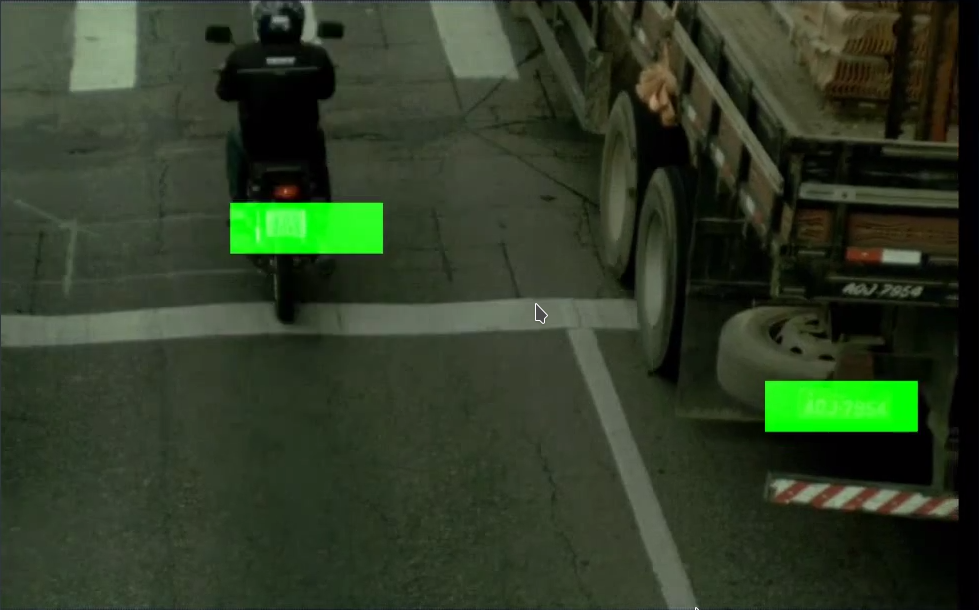
\includegraphics[scale=0.3]{cap1_resultado_esperado.png}
	\caption{Resultado esperado}
	\label{fig:cap1_resultado_esperado}
	(próprio autor).
\end{figure}

Soluções de monitoração e fiscalização de veículos apresentam
uma grande demanda por sistemas de visão computacional. Seja
para contar tráfego, fiscalizar o uso das vias, monitorar
rodízios ou para cobrar pedágios, a capacidade de obter
informações a partir de imagens é de grande interesse, sendo parte integrante
de uma solução típica \cite{anagnostopoulos2008license}.  Existem
soluções propostas para parte destes problemas, no entanto há a
possibilidade da busca por estratégias com menor custo ou melhor
desempenho, à medida que avanços no campo do reconhecimento de
imagens acontecem.

Redes neurais convolucionais (\sigla{CNN}{\emph{Convolutional neural network},
rede neural convolucional}, convolutional neural networks)
são tipos de redes neurais biologicamente inspiradas no conceito
de campos receptivos \cite{hubel1968receptive}. Este tipo de
rede viabilizou o uso de redes neurais que são alimentadas
diretamente pelos \emph{pixels} da imagem \cite{lecun1998gradient}. O
advento das Redes Neurais Convolucionais Profundas (\sigla{DCNN}{\emph{Deep
convolutional neural network}, rede neural convolucional profunda}, deep CNN)
viabilizou um grande salto na capacidade de sistemas computacionais
de classificação. O uso de mais camadas permite níveis maiores de
abstração na análise da imagem, o que resulta em maior taxa de
acerto, ao custo de maior tempo de treinamento. Este tipo de rede
neural representa o atual estado-da-arte em reconhecimento de
imagens \cite{szegedy2015going}.

Este projeto procura fazer aplicação direta de DCNN para localizar
placas de veículos em vídeos como forma de produzir um sistema
robusto, flexível, e de alto desempenho.

\section{Objetivo}
O objetivo deste trabalho é desenvolver uma abordagem para
treinamento e uso de redes neurais convolucionais para para a
construção de um sistema robusto e eficiente de localização de
placas de veículos em vídeo, e realizar uma implementação para
medição de dados de desempenho.

\section{Estrutura da Monografia}
O restante deste trabalho é organizado da seguinte forma: O
capítulo 2 discorre sobre redes neurais convolucionais em geral,
comparando-as com as redes neurais não-convolucionais. Como este
tópico é relativamente novo optou-se por fazer sua apresentação
o mais cedo possível no documento. O capítulo 3 é uma revisão da
bibliografia atual sobre detecção e localização de placas veiculares. O
capítulo 4 apresenta uma proposta de um método para aplicar redes neurais
convolucionais para localizar placas veiculares. O capítulo 5 apresenta uma
implementação do método proposto, experimentos e os seus resultados. O
capítulo 6 apresenta as conclusões deste trabalho.

 % introdução
%Exemplo de capitulo

\chapter{Redes Neurais Convolucionais}
\setcounter{figure}{100}

Rede neural artificial (\sigla{ANN}{\emph{Artificial Neural Network},
rede neural artificial}) é um modelo computacional inspirado na forma com
que o cérebro resolve problemas \cite{gilbert2000build}. Este modelo possui
unidades, denominadas neurônios, que possuem um valor que é calculado como uma
função do valor de outros neurônios.

\begin{figure}[!htb]
	\centering
	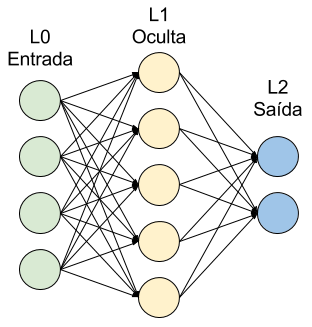
\includegraphics{ex_fcnn.png}
	\caption{Exemplo de rede neural totalmente conectada}
	\label{fig:ex_fcnn}
	(próprio autor).
\end{figure}

Alguns neurônios especiais, denominados “entradas” possuem um valor obtido de
fora do sistema. Estes são especiais porque são os únicos cujos valores não são
calculados. O valor de alguns dos neurônios de uma rede neural artificial podem
afetar sistemas externos à ela. Por isso são designados “saídas”. Neurônios que
não são de entrada ou de saída são chamados “ocultos”. A figura
\ref{fig:ex_fcnn} ilustra uma rede neural simples com os três tipos de
neurônios.

\section{Redes Neurais Não-Convolucionais}
As redes neurais artificiais são tipicamente organizadas em “camadas”, e a
escolha dos tipos de neurônio, juntamente com a forma com que os neurônios são
conectados, é denominada “topologia”. As redes são classificadas como
feedforward quando as conexões não formam ciclos ou recurrent quando formam. Se
uma camada está conectada a todos os neurônios da camada anterior diz-se que a
camada é totalmente conectada.
A definição da função de transferência do neurônio é uma parte importante da
topologia das redes neurais. Um tipo muito comum de neurônio é definido por:

\begin{equation} \label{eq:non-conv-layer}
	v=A \left( \left( \sum_n w_n i_n \right) + b \right)
\end{equation}

Onde $v$ é o valor do neurônio, $i_n$ é n-ésima entrada do neurônio,
$w$ é um vetor de escalares denominado peso, e $b$ é um escalar arbitrário,
denominado bias. A é uma
função denominada função de ativação do neurônio. Essa função pode ser usada
para tornar o neurônio não-linear, como no caso da tangente hiperbólica. Os
pesos determinam a influência de cada entrada do neurônio.

A descrição de redes neurais com este tipo de neurônio e com topologia
totalmente conectada é especialmente conveniente. As três camadas
da rede neural ilustrada na figura \ref{fig:ex_fcnn} podem ser representadas
por matrizes:

\noindent\begin{minipage}{.333\linewidth}
	\begin{equation} \label{eq:l0}
		L0_{4 \times 1} =
			\begin{pmatrix}
				a_1 \\
				a_2 \\
				a_3 \\
				a_4
			\end{pmatrix}
	\end{equation}
\end{minipage}
\begin{minipage}{.333\linewidth}
	\begin{equation} \label{eq:l1}
		L1_{5 \times 1} =
			\begin{pmatrix}
				b_1 \\
				b_2 \\
				b_3 \\
				b_4 \\
				b_5
			\end{pmatrix}
	\end{equation}
\end{minipage}
\begin{minipage}{.333\linewidth}
	\begin{equation} \label{eq:l2}
		L2_{2 \times 1} =
			\begin{pmatrix}
				c_1 \\
				c_2
			\end{pmatrix}
	\end{equation}
\end{minipage}

Para calcular a primeira camada intermediária é preciso aplicar a equação
(\ref{eq:non-conv-layer}) cinco vezes, uma para cada neurônio. Porém, se
esta camada for totalmente conectada, e todos os neurônios usarem a
mesma função de transferência $A$, e a representação em matrizes estiver
sendo usada, o cálculo de todos os neurônios desta camada pode ser
realizado usando:

\begin{equation}
	L1_{5 \times 1}=A_V \left( W1_{5 \times 4} \times L0_{4 \times 1}
		+ B1_{5 \times 1} \right)
\end{equation}

Onde $A_V$ é uma versão vetorial da função de ativação resultante
da aplicação da função $A$ em cada um dos elementos do vetor.
Os pesos dos cinco neurônios, denominados $w_n$ na equação
\ref{eq:non-conv-layer} são aqui representados por uma única matriz
$W1_{5 \times 4}$, e os bias dos cinco neurônios, $b$, são representados por
uma única matriz $B1_5$. Da mesma forma, a camada de saída
pode ser calculada com:

\begin{equation}
	L2_{2 \times 1}=A_V \left( W2_{2 \times 5} \cdot L1_{5 \times 1}
		+ B2_{2 \times 1} \right)
\end{equation}

As matrizes $W$ e $B$ são os parâmetros que precisam ser aprendidos durante o
treinamento, e são denominados parâmetros treináveis. O número de parâmetros
de uma uma
rede neural é igual ao número de valores contidos em todas as matrizes de pesos
e bias. Quanto maior o número de parâmetros, mais flexibilidade a rede neural
possui, porém mais lento é o treinamento. Se o número de parâmetros for
excessivo a rede neural perde a capacidade de generalizar e ocorre
\emph{overfitting}.

De acordo com \cite{hawkins2004problem}, \emph{overfitting} ocorre quando um
modelo é mais flexível do que precisa ser. Quando um modelo destes é treinado,
especialmente com poucos exemplos, o modelo pode acabar "memorizando" os
exemplos, ao invéz de generazar o comportamento geral dos dados, fazendo
com que o resultado da classificação seja bom, mas haja erro excessivo
quando o mesmo modelo é aplicado em dados novos.

Como as dimensões da matriz de pesos são iguais ao número de entradas em uma
direção pelo número de saídas na outra direção, o número de parâmetros nessa
matriz é igual ao produto dos dois. Se uma camada totalmente conectada tem 1000
entradas e 1000 saídas a matriz de pesos vai possuir 1.000.000 de parâmetros
e a matriz de \emph{bias} mais 1.000, resultando em um total de 1.001.000
parâmetros.

\section{Redes Neurais Convolucionais}
Redes neurais convolucionais são um tipo de rede neural que inclui operações
baseadas em uma definição relaxada de convolução. A principal operação
neste tipo de rede neural é a a correlação cruzada (\emph{cross-correlation}).
Para duas funções discretas $f$ e $g$, a correlação cruzada discreta entre
elas é definida por:

\begin{equation}
	def: (f \star g)[n] = \sum_{m=-\infty}^{\infty} f^*[m]g[m+n]
\end{equation}

Onde $f^*$ é o complexo conjugado da função $f$. A figura
\ref{fig:cap2_ex_corr_cruz_1d} ilustra uma operação de correlação cruzada sendo
realizada pelo método visual.

\begin{figure}[!htb]
	\centering
	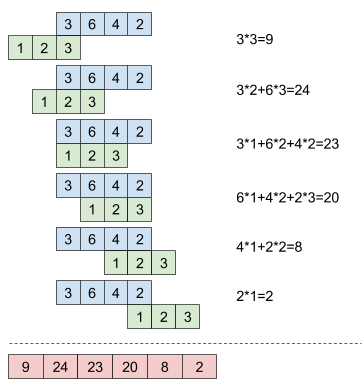
\includegraphics{cap2_ex_corr_cruz_1d.png}
	\caption{Exemplo de correlação cruzada 1D}
	\label{fig:cap2_ex_corr_cruz_1d}
	Na imagem está sendo calculada a correlação cruzada entre [3,6,4,2] e
	[1,2,3]. O primeiro set de dados fica fixo enquanto o segundo vai sendo
	deslocado, e em cada vez se calcula a soma do produto, conforme ilustrado.
	O resultando é [9,24,23,20,8,2].
\end{figure}

A correlação cruzada também é definida para dimensões maiores que 1.
Tomando as funções discretas $f[n_1,n_2]$ e $g[n_1,n_2]$ pode-se 
escrever a convolução 2D destas funções como sendo:

\begin{equation}
	def: (f \star\star g)[n_1,n_2] =
		\sum_{m_1=-\infty}^{\infty} \quad
		\sum_{m_2=-\infty}^{\infty}
		f^*[m_1,m_2]g[m_1+n_1,m_2+n_2]
\end{equation}

É possível realizar convoluções para um número arbitrário de dimensões através
da generalização desta equação.

A aplicação do operador de correlação cruzado é próximo ao conceito de filtro
linear, bastante usado em processamento digital de imagens
\cite{gonzalezwoods200708}. Os conceitos não
são idênticos por que filtro digital trata uma das entradas como sendo "sinal",
e a outra como sendo o filtro, ou \emph{kernel}, e convoluções e correlações
cruzadas tratam as duas entradas de forma idêntica, e produzem um resultado
diferente nos extremos. Como observa-se na figura
\ref{fig:cap2_ex_corr_cruz_1d}, a saída é um vetor de dimensão 6, e um filtro
digital geraria saída de tamanho 4 (se houvesse extensão de borda).
No entanto, os resultados são idênticos para as saídas onde todos os membros
das duas entradas possuem um par na outra entrada. Mais detalhes sobre isso
serão cobertos na sessão \ref{ses:bordas}.

A correlação cruzada entre $f[n]$ e $g[n]$
é igual a convolução entre $f[n]$ e $g[-n]$, e relações semelhantes existem
para qualquer dimensionalidade. Uma camada de uma rede
neural que use qualquer uma das operações é denominada “convolucional”,
pois neste contexto as operações são intercambiáveis. Como $g$ vai
representar os parâmetros treináveis. Ao se trocar convolução por correlação
cruzada os mesmos parâmetros serão aprendidos em uma ordem diferente.
Por este motivo os termos "convolução" e "convolucional" são usados de forma
relaxada no contexto de redes neurais. Conforme será visto adiante, existe
mais um motivo para isso.

O uso de convoluções em redes neurais, especialmente para dimensões superiores
a 1, requerem que os dados nos quais este operador vai ser executado sejam
representados de forma a preservar o posicionamento dos valores.

Uma das formas de estruturar os dados é usando tensores, que são uma
extensão de
vetores que admite um número arbitrário de dimensões. O motivo para isso é
permitir preservar a geometria da informação que está sendo processada.

Se a rede neural convolucional for ser aplicada em uma
imagem bidimensional com dimensões $H$ e $W$ com C canais de cor, ela pode ser
representada por um tensor de dimensões $H \times W \times C$. Uma imagem
tridimensional com profundidade $D$ é representada por um tensor
$D \times H \times W \times C$, e assim por
diante. Isso permite preservar o posicionamento relativo das informações
e viabiliza aplicar o operador de correlação cruzada.

A ordem das dimensões dos tensores não precisa ser necessariamente a que está
descrita aqui. Nas implementações concretas de softwares de redes neurais os
desenvolvedores podem escolher, até certo ponto, a ordem que irão usar baseado
em fatores diversos, como arquitetura das GPUs onde o software vai rodar. Aqui
está sendo adotada a ordem padrão do \emph{TensorFlow}.

Caso a rede neural esteja operando sobre um tipo de informação que não possui o
conceito de “canal”, como séries temporais, é conveniente artificialmente
criá-lo. Esse é o caso de séries temporais com “N” entradas, que serão
representadas por um tensor com dimensões $N\times1$. O motivo para isso é
uniformidade. O tensor de saída de uma camada convolucional inclui a dimensão
“canal”. Forçando tanto os tensores de entrada quanto de saída a incluírem um
canal, o mesmo conceito de camada convolucional é aplicável em todas as camadas
com o mesmo número de dimensões.

Uma camada convolucional é definida pela a aplicação de um \emph{kernel} sobre
a entrada dessa camada usando o operador convolução. Como já foi mencionado,
o uso do termo convolução
é bastante relaxado neste caso por que, além de normalmente referir-se a
uma correlação cruzada, é aplicado de forma idêntica à aplicação de um filtro
digital, gerando as diferenças já discutidas no resultado.

O filtro da camada convolucional é um tensor que contém parâmetros treináveis.
Se a entrada da camada convolucional tem dimensões
$D0 \times D1 \times D2 \times ... \times C$, onde C é o número de canais,
o filtro terá o mesmo número de dimensões, sendo que o tamanho de todas
as dimensões, exceto a última são
hiperparâmetros arbitrários. A última dimensão do filtro precisa ser igual ao
número de canais da imagem de entrada da camada convolucional, como ilustrado na
figura \ref{fig:ex_conv_2d}.


\begin{figure}[!htb]
	\centering
	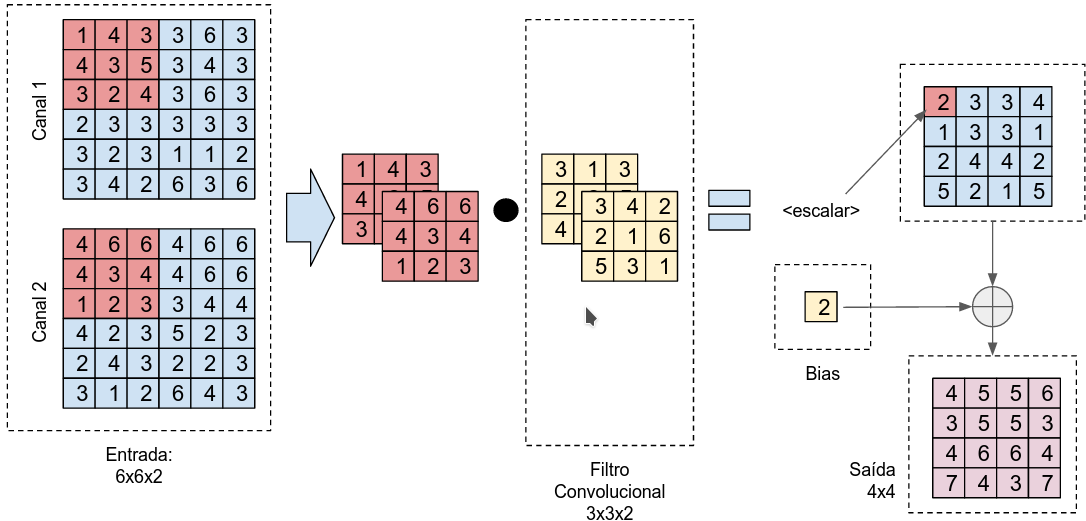
\includegraphics{ex_conv_2d.png}
	\caption{Exemplo de convolução 2D}
	\label{fig:ex_conv_2d}
	Exemplo da aplicação de uma única convolução sendo aplicada a uma imagem de
	entrada $6 \times 6 \times 2$. O tamanho da última dimensão do filtro e
	da entrada precisam ser iguais, no caso 2. As dimensões $3 \times 3$ do
	filtro foram escolhidas arbitrariamente. O símbolo do círculo na imagem
	representa um produto interno. A imagem de saída foi gerada deslocando
	a seleção de pixel a pixel até cobrir toda a
	imagem de entrada. Como as bordas não foram estendidas, a imagem
	resultante é menor que a de entrada (próprio autor).
\end{figure}

Camadas convolucionais também usam o conceito de bias. Para isso o tensor
resultante da convolução é somado a um escalar. Este escalar é treinável e
permite, entre outras coisas, que a rede neural gere valores não-nulos mesmo que
a entrada seja nula.

\subsection{Bordas} \label{ses:bordas}
Como já foi mencionado, a convolução é aplicado de forma idêntica a aplicação
de um filtro linear \cite{gonzalezwoods200708}, e assim como no caso dos
filtros lineares, existem algumas opções para tratamento de bordas dos dados.

Na figura \ref{fig:ex_conv_2d} o tamanho do tensor de saída foi reduzido
de 6 para 4. Neste caso a opção foi por não extender as bordas. Por
este motivo, o resultado tem que ser reduzida para impedir que o filtro
possua termos despareados.

Pode ser
desejável fazer a saída ter o mesmo tamanho da entrada. Para isso é necessário
estender as bordas da entrada, o que permitiria ao filtro ser deslocado por
toda a extensão entrada. Em camadas convolucionais observou-se apenas a
extensão com zeros. O software que foi adotado para a implementação deste
trabalho não suporta extensão que não seja com zeros, e não foi encontrado
\emph{paper} usando método diferente, como repetição.

A opção de extensão de borda é um hiperparâmetro.

\subsection{\emph{Stride}}
Ao se aplicar o filtro de convolução no tensor de entrada pode-se movê-lo de
posição a posição, até cobrir todos os locais válidos em cada direção, como
ilustrado na figura \ref{fig:ex_conv_2d}, ou pode-se desejar aplicar a cada
"$n_0$" pixels em uma direção, “$n_1$” pixels em outra direção, e assim por diante.
Esta opção é denominada \emph{stride}.

Quando uma camada convolucional possui como entrada um tensor de dimensões
$d1\times d2 \times ... \times dj \times C$, o stride é definido como sendo
um tensor unidimensional de tamanho j.
O stride $[1,2,1]$, por exemplo, indica que na primeira dimensão o
filtro será aplicado em todas as posições válidas, na segunda dimensão será
aplicado a cada 2 pixels e na terceira será aplicada novamente em todas as
posições válidas. Stride maior que 1 causa redução no tamanho do tensor de
saída.

Se um stride $2 \times 2$ fosse aplicado na convolução da figura
\ref{fig:ex_conv_2d} a imagem de saída seria $2 \times 2$.

\subsection{Profundidade do Filtro}
A figura \ref{fig:ex_conv_2d} mostrou um único filtro sendo aplicado ao
tensor de entrada. No
entanto, é possível aplicar um número arbitrário deles, sendo que cada filtro
produz um tensor de saída.

\textbf{Neste ponto, falar isso fica meio sem sentido. Como assim, "reconhecer
feature"? O que isso quer dizer? Seria melhor expandir um pouco mais a
descrição em algum ponto, para indicar que um neurônio de uma camada
convolucional produz uma resposta a algum tipo de característica. Nas primeiras
camadas, normalmente são primitivas simples, como segmentos de reta, pontos
isolados, e formas simples. Em camadas mais profundas, estas primitivas vão
sendo recombinadas, resultando me featuers mais complexas. Não sei se é melhor
falar disso antes ou DEPOIS daqui. Mas uma hora, isso precisa ser dito.}

Se o tensor de entrada possui dimensões $d0 \times d1 \times ... \times C$
e deseja-se aplicar sobre este
tensor $N$ convoluções é possível representar isso com um único tensor
com dimensões
$N \times d0 \times d1 \times ... \times C$. Cada um dos filtros vai gerar
um tensor de saída, em um total de $N$. O
número de filtros é denominado “profundidade do filtro”. Todas as saídas podem
ser representadas em um único tensor com uma dimensão adicional. Usa-se a última
dimensão do tensor de saída para este fim. O motivo para isso é que cada uma
dessas saídas efetivamente se torna um “canal” de saída desta rede neural. No
exemplo da figura \ref{fig:ex_conv_2d}, se fossem aplicados 3 filtros a saída
seria um tensor $4 \times 4 \times 3$. Para isso o tensor que define o filtro
convolucional passaria a ser um
filtro de profundidade 3 descrito por um tensor de dimensões
$3 \times 4 \times 4 \times 2$.

\subsection{Processamento em Lotes}
Existem alguns cuidados especiais que devem ser tomados durante o treinamento de
redes neurais. Tomando o caso do treinamento supervisionado como exemplo, o
otimizador ajusta os parâmetros treináveis da rede neural para tentar reduzir o
erro. Para verificar se a alteração teve sucesso, a rede neural é
alimentada com
dados rotulados, e o valor de saída da rede neural é comparado com os dados
esperados. É conveniente fornecer vários exemplos rotulados, não apenas um, e
usar a média do erro para alimentar o otimizador. A ideia é que o valor passado
seja o mais representativo possível.

O número de imagens fornecidas é denominado "tamanho do lote". Se uma rede
neural trabalha com dados de dimensões $d0 \times d1 \times ... \times C$
podem-se agrupar “B” exemplos em
um único tensor, com dimensões $B \times d0 \times d1 \times ... \times C$.
As camadas convolucionais tratam cada
uma das imagens separadamente, conforme já foi descrito, e emite na sua saída um
único tensor que também usa uma dimensão adicional para agrupar as diferentes
imagens.

O valor de B não é um hiperparâmetro, mas sim um parâmetro de treinamento.

\subsection{Pooling}
Após a aplicação de uma camada convolucional pode-se aplicar uma camada de
\emph{pooling}, que é uma forma de subamostragem. A figura
\ref{fig:ex_maxpool} ilustra uma operação de maxpool, que é um tipo de
pooling.

\begin{figure}[!htb]
	\centering
	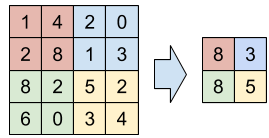
\includegraphics{ex_maxpool.png}
	\caption{Exemplo de \emph{maxpool} $2 \times 2$}
	\label{fig:ex_maxpool}
	Ilustração de uma operação maxpool $2 \times 2$ aplicado usando stride
	$2 \times 2$. O filtro move de dois em dois pixels e possui
	tamanho 2 em cada dimensão (próprio autor).
\end{figure}

Esta operação possui como parâmetros o tamanho do filtro, o stride e a opção de
borda. A operação a ser aplicada no filtro pode ser $max$ ou $avg$ (média),
que definem respectivamente os filtros \emph{maxpool} e \emph{avgpool}.

Como as operações de pooling são normalmente feitas com stride maior que 1 elas
acabam reduzindo consideravelmente o tamanho do tensor de saída. No caso de um
maxpool $2 \times 2$, por exemplo, o tensor resultante vai ter 25\% do
número de valores do tensor de entrada.

Uma camada convolucional com pooling pode ser contada como uma única camada ou
como duas, dependendo do caso. Em algumas arquiteturas mais complexas, como em
\cite{szegedy2015going}, onde define-se camadas do tipo \emph{inception},
pode não ser possível associar uma operação de \emph{pooling} a uma única
convolução, requerendo contagem separada.

\subsection{ReLu}
Assim como em redes neurais totalmente conectadas, pode-se aplicar uma função
de ativação para tornar a camada não-linear. As funções tangente
hiperbólica, sigmóide ou outras tipicamente usadas em redes neurais
não-convolucionais podem ser aplicadas. No entanto a função
\sigla{ReLu}{\emph{Rectified linear}, linear retificada}, ou linear
retificada, resulta em treinamento substancialmente mais rápido enquanto
mantém a capacidade de generalização da rede neural treinada. A função
ReLu é definida por:


\begin{equation}
	ReLu(x) = max(0,x)
\end{equation}

Quando uma camada de uma rede neural inclui apenas elementos lineares,
ela é dita linear. O operador de convolução em sí é linear, então
isso vai ocorrer quando a camanda não inclui uma função de ativação, como
a ReLu e não possui outros elementos não-lineares, como \emph{maxpool},
caso o pooling esteja sendo considerado como parte da camada convolucional.

\subsection{Últimas Camadas}
Após as camadas convolucionais terem sido aplicadas é necessário usar um
classificador, mecanismo de regressão ou outro sistema que gere o tipo de saída
desejada para a rede neural. Uma das possíveis formas de realizar esta função é
usar uma ou duas camadas totalmente conectadas, como ilustrado na figura
\ref{fig:ex_cnn}. No exemplo a função de ativação da penúltima camada é
ReLu e a última camada é linear.

\subsection{Rede Neural Convolucional Completa}
Para alguns casos simples, pode-se construir uma rede neural convolucional
conectando-se uma camada convolucional a uma maxpool e uma ReLu. Este conjunto
pode ser repetido algumas vezes até que o número de saídas da camada
convolucional seja baixo o suficiente para que seja passado por duas camadas
totalmente conectadas. Se houver interesse em não reduzir o tamanho total do
tensor pode-se omitir a camada \emph{maxpool}. Um exemplo dessa topologia é a
figura \ref{fig:ex_cnn}.

A primeira camada da rede neural vai ter filtros que serão sensíveis a
características simples da entrada, que no caso de imagens seriam, por exemplo,
gradientes e trechos de linhas. Em
cada camada seguinte estas características são recombinadas com as detectadas
nas regiões vizinhas, formando conceitos progressivamente mais sofisticados a
respeito da imagem.

A topologia da rede neural e o conjunto de todos os hiperparâmetros definem o
número de parâmetros treináveis que a rede neural vai possuir e quantas
operações são necessárias para aplicar a rede neural em um (ou um lote de)
amostras. Uma rede neural mais larga, com um maior número de filtros por
camadas, possui a capacidade de aprender mais \emph{features}. Redes neurais
mais profundas possuem capacidade de abstração maior, sendo capazes de inferir
a partir dos dados de entrada conceitos mais complexos.

\begin{figure}[!htb]
	\centering
	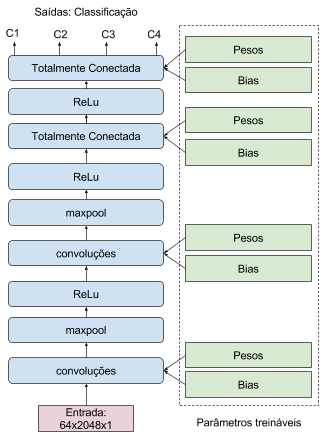
\includegraphics{ex_cnn.png}
	\caption{Exemplo de rede neural convolucional completa}
	\label{fig:ex_cnn}
	Esta rede neural possui nove camadas para
	classificação de séries temporais em uma de 4 classes. Destacam-se os
	parâmetros treináveis (próprio autor).
\end{figure}

\section{Uso em Processamento de Imagens}
O uso de redes neurais convolucionais é uma alternativa a diversos métodos já
existentes de detecção e reconhecimento de objetos em imagens. Aqui serão
mostradas algumas das alternativas usuais, para que sejam contrastadas
com a classificação baseada em redes neurais convolucionais.

\subsection{Redes Neurais Não-Convolucionais}
Quando uma imagem vai ser processada por uma rede não-convolucional ela precisa
ser convertida para a forma plana, em um vetor com dimensões
$H \cdot W \cdot C \times 1$.

O uso de camadas totalmente conectadas é proibitivo para classificação de
imagens desta maneira. Se uma rede neural for usada para processar imagens de 1
megapixel, ou $720 \times 1280$, e a primeira camada possuir um
número de neurônios igual
ao número de neurônios da camada de entrada, a matriz de pesos teria
$(720 \cdot 1280 \cdot 3)^2 \approx 7.6 \cdot 10^{12}$ parâmetros. Se for
representado por números ponto-flutuante de 32 bits isso ocuparia mais de
30 TiB. O mesmo processo em uma imagem 480px por 640px geraria quase 850
bilhões de parâmetros só na matriz de pesos.

Outras topologias mais esparsas podem ser construídas, mas este tipo de rede
neural possui outros problemas que as tornam inviáveis para processamento direto
de imagens. Um exemplo é o fato delas não serem invariantes ao deslocamento. Se
a rede neural aprende a reconhecer um \emph{feature} em um local da
imagem, não vai
conseguir reaproveitar essa capacidade em outras posições. Portanto teria que
aprender a mesma \emph{feature} em cada possível posição onde ela possa
aparecer, e fazer isso para todas as \emph{features}.

Como a primeira operação feita foi converter a imagem para um formato “plano”, a
geometria da imagem foi destruída. Não é mais possível determinar quando dois
pixels estão próximos, e essa é uma informação muito importante sobre a imagem.

\subsection{Uso de descritores}
Uma das abordagens possíveis para reconhecimento e detecção de imagens é o uso
de descritores. Esta foi a abordagem dominante até pouco tempo atrás.

Os descritores são operações que tomam uma imagem como entrada e resumem as sua
características em um set menor de informações. Exemplos de descritores muito
usados são \sigla{LBP}{Local binary patterns} \cite{wang1990texture},
\sigla{ORB}{Oriented FAST and rotated BRIEF} \cite{rublee2011orb},
\sigla{HOG}{Histogram of oriented gradients} \cite{dalal2005histograms},
Haar-Wavelets \cite{nabout2008object},
filtros de Gabor \cite{riaz2012invariant}. O treinamento é realizado sobre
as features extraídas pelo descritor escolhido usando um classificador como
redes neurais ou \sigla{SVM}{\emph{Support vector machine}}.

Para usar esta abordagem um descritor precisa ser escolhido e configurado,
muitas vezes manualmente. O desempenho do sistema como um todo vai depender
dessas escolhas. Se a operação de detecção depender de conceitos complexos,
envolvendo correlação entre múltiplas características, o descritor e o
classificador precisam ser escolhidos especificamente para isso.

\subsection{Redes Neurais Convolucionais em Imagens}
As redes neurais convolucionais operam diretamente nos pixels da imagem, não
sendo necessário escolher um descritor, e não possuem os problemas que as
redes não-convolucionais possuem. As camadas convolucionais se comportam como
descritores, porém os parâmetros são aprendidos como parte do processo de
treinamento, portanto são otimizados para responderem precisamente para os
exmeplos que forem fornecidos. Apenas alguns hiperparâmetros, como tamanho
da convolução, número de filtros e de camadas precisam ser escolhidos mediante
decisões de meta de precisão e recall, tempo para classificação e complexidade
dos conceitos a serem aprendidos.

As redes neurais convolucionais resolvem todos esses problemas simultaneamente.
O primeiro ponto é a preservação da geometria da imagem. Se uma imagem de 50
pixels de altura por 100 pixels de largura contendo 3 canais de cor for usado na
entrada de uma rede neural convolucional, ela precisa ser representada por um
tensor apropriado, como $32 \times 50 \times 100 \times 3$. Este tensor
permite alimentar a rede neural com um lote de 32 imagens.

Para aplicar uma camada convolucional à imagem de entrada escolhe-se o tamanho
da convolução, o número de filtros e o modo de operação nas bordas. A figura
\ref{fig:ex_cnn_img} ilustra um filtro 33 sendo aplicado a uma imagem
\sigla{RGB}{\emph{Red, green, blue}, vermelho, verde, vermelho}.

\begin{figure}[!htb]
	\centering
	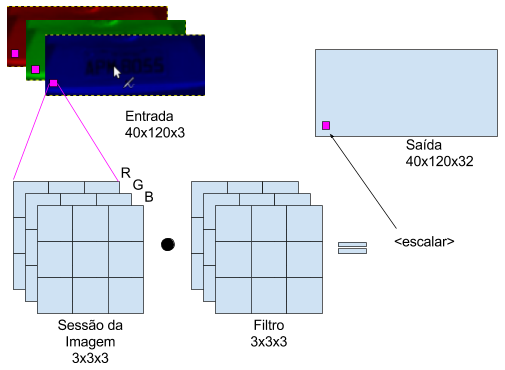
\includegraphics{ex_cnn_img.png}
	\caption{Convolução sendo aplicada em uma imagem RGB}
	\label{fig:ex_cnn_img}
	Como a imagem possui 3 canais o filtro será $3 \times 3 \times 3$.
	Uma partição da imagem original com o mesmo tamanho do filtro,
	$3 \times 3 \times 3$ é extraído da imagem, e um
	produto interno é realizado entre os dois, resultando em um escalar. Este
	escalar é armazenado no tensor de saída nas coordenadas corretas. A
	ilustração só mostra uma imagem de entrada e só um filtro e, portanto, uma
	imagem de saída (próprio autor).
\end{figure}

Para que o filtro tenha profundidade 64, por exemplo, o tensor que define o
filtro será $64 \times 3 \times 3 \times 3$ e o tensor resultante da
convolução será $32 \times 40 \times 120 \times 64$,
considerando que seja usado preenchimento nas bordas.

Para finalizar a camada convolucional adiciona-se um bias. Para isso usa-se um
escalar para cada uma das 64 imagens resultantes. O tensor que define os bias é
um tensor unidimensional com tamanho 64.

Camadas maxpool e ReLu podem ser adicionadas para reduzir as dimensões da imagem
ou aumentar a sua não-linearidade. A figura \ref{fig:ex_full_cnn_img}
ilustra o uso das três camadas em sequência.

\begin{figure}[!htb]
	\centering
	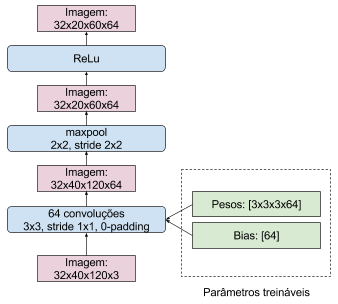
\includegraphics{ex_full_cnn_img.png}
	\caption{Exemplo de rede neural convolucional completa aplicada à uma imagem
	RGB}
	\label{fig:ex_full_cnn_img}
	Exemplo de uma sequência de operações feitas usando uma rede neural
	convolucional incluindo 64 convoluções $3 \times 3$, maxpool e ReLu
	aplicadas em uma
	lote de 32 imagens $40 \times 120 \times 3$. Os parâmetros treináveis
	estão destacados (próprio autor).
\end{figure}

A imagem é tratada por camadas sucessivas de convolução, maxpool e ReLu até que
o tamanho total do tensor seja pequeno o suficiente para poder ser processado
por duas camadas totalmente conectadas. 

\subsection{Uso de Cores}
Em alguns sistemas de visão computacional são usadas imagens em
tons de cinza. No caso de redes convolucionais o mais comum é usar
imagens coloridas.

O primeiro motivo para isso é que as imagens e vídeos são normalmente
captadas com cores, então o processo de detecção teria que incluir uma operação
de conversão para escala de cinza. 

Pode-se demonstrar todos os métodos de conversão lineares de RGB para escala de
cinzas, como:

\begin{equation} \label{eq:rgb2gray}
	G=0.299R + 0,587G + 0.114B
\end{equation}

Podem ser representados como uma convolução $1 \times 1$. Visto que as
convoluções são implementadas de forma bastante eficientes nas bibliotecas
de redes neurais convolucionais, algumas vezes até usando aceleração por
hardware, então não necessariamente haverá economia durante a execução
durante a execução da rede neural, pois, no pior caso, ela mesma pode fazer
essa conversão de forma eficiente, sendo que os coeficientes associados
à cada canal, que no exemplo da equação \ref{eq:rgb2gray} são fixos, podem
treinados pelo otimizador, potencialmente obtendo uma conversão mais apropriada
para a rede neural.

Outro ponto é que os sistemas que representam o atual
estado-da-arte para reconhecimento de imagem, como \cite{szegedy2015going}
\cite{hasanpour2016lets}, usam cores, portanto nos casos onde
existe \emph{budget} computacional, e particularmente quando é possível usar
vários filtros convolucionais na primeira camada, a informação da cor pode
ser vantajosa para para minimizar os erros da rede neural.

\subsection{Reconhecimento de Objetos}
Existem várias maneiras de se usar redes neurais para reconhecer objetos. Duas
das opções envolvem configurar a neural como classificador e como sistema de
regressão.

Para usar a rede como classificador pode-se incluir na última camada da rede
neural um sistema softmax, também conhecido como exponencial normalizada. Isso
permite que a rede neural seja treinada e, após o treinamento, estime a
probabilidade da sua entrada pertencer a cada uma de N classes. A rede neural é
implementada usando $N$ saídas, de forma que cada saída é treinada para
representar a probabilidade da entrada ser classificada em em uma das classes.
Uma saída \emph{softmax} realiza uma normalização das saídas da rede neural,
usando a equação:

\begin{equation}
	softmax[i] = \frac
		{exp\left( \widehat{out}[i] \right)}
		{\sum_j exp\left( \widehat{out}[j] \right)}
\end{equation}

Para identificar a presença ou não do objeto que está sendo procurado, duas
classes seriam definidas: "presente" e "não-presente", resultando em uma rede
neural como mostrada na figura \ref{fig:ex_classif_logist}.

\begin{figure}[!htb]
	\centering
	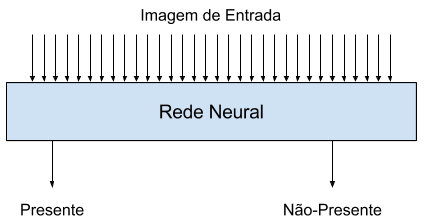
\includegraphics{ex_classif_logist.png}
	\caption{Exemplo de Classificador Logístico}
	\label{fig:ex_classif_logist}
	Este exemplo de rede neural possui uma imagem como entrada e possui duas
	saídas, uma informando a probabilidade da imagem conter o objeto, outra
	indicando a probabilidade de não conter (próprio autor).
\end{figure}

Este modelo pode ser treinado usando modo supervisionado, onde imagens
pré-classificadas são fornecidas. A função de perda a ser minimizada pelo
otimizador é a função \emph{cross entropy}:

\begin{equation}
	\widehat{H} = - \sum_i \widehat{y_i} log(y_i)
\end{equation}

Onde $y_i$ é o valor da probabilidade manualmente
marcadas de uma imagem pertencer à classe $i$ (no caso, a probabilidade de ser
uma imagem que contém o objeto e a probabilidade não conter) e $\widehat{y_i}$
é o valor estimado pela rede neural. $H$ é o valor estimado de
\emph{cross entropy}.

Quando têm-se o objeto desejado centrado na imagem, ou o objeto não consta
em lugar nenhum da imagem usa-se os valores $0$ e $1$ para rotular os exemplos.
Os casos onde o objeto está visível apenas parcialmente deve ser considerado
cuidadosamente, produzindo valores intermediários nos rótulos, para evitar que
duas imagens parecidas gerem valores muito diferentes na saída da rede neural.

As redes neurais também podem ser usadas para fazer regressão, ou seja, modelar
uma função. A forma mais óbvia de implementação é a regressão L2. Neste tipo de
função o otimizador vai minimizar o erro quadrático:

\begin{equation}
	E=\left( y - \widehat{y} \right)^2
\end{equation}

A rede neural pode ser usada para modelar a função $P$, definida por:

\begin{equation}
	P(img) = \begin{cases}
		1 \text{, se img contém o objeto procurado} \\
		0 \text{, se img não contém}
	\end{cases}
\end{equation}

Exatamente essa definição não seria ideal, pois não considera placas visíveis
parcialmente. Em uma implementação real de classificador baseado neste método
precisa definir uma função que seja contínua em resposta ao objeto é movido do
centro da imagem para fora por qualquer caminho.

\subsection{Localização de Objetos} \label{sec:localiz_objetos}
Até agora foi mostrado como usar redes neurais convolucionais para detectar um
objeto em uma imagem. Isso envolve apenas determinar se uma imagem possui ou não
o objeto de interesse. Localização, ao contrário, requer a determinação das
coordenadas do objeto.

Um sistema de localização pode ser construído a partir de um sistema de
detecção. A abordagem mais simples para isso envolve construir um sistema capaz
de detectar o objeto de interesse e aplicar este
detector à imagem várias vezes a imagem usando "janelas deslizantes".
Se o detector for construído para produzir “1” quando detectar o objeto e
“0” então os pontos de máxima são candidatos a centros dos objetos.

Como cada pixel da imagem é candidato a centro do objeto que está sendo
localizado, deve-se aplicar o filtro uma vêz para cada pixel. Se não houver
extensão de bordas, o filtro não pode ser aplicado em parte dos pixels.
 % redes neurais convolucionais
%Exemplo de capitulo

\chapter{Trabalhos Relacionados}

\section{Redes neurais convolucionais aplicadas a imagens}

Comparação direta entre diferentes abordagens para reconhecimento e detecção de
imagem podem ser realizadas se um conjunto de dados comum e suficientemente
grande for usado. A competição \emph{ILSVRC, ImageNet Large Scale Visual
Recognition Challenge} é uma competição que ocorre anualmente desde 2010, e é
voltada a este fim. Esta competição permite comparar soluções 
para diferentes problemas, como classificação de imagens e localização de
objetos em um conjunto de
de dados contendo milhões de imagens manualmente rotuladas entre centenas de
categorias. O set de dados está disponível publicamente, e existe um
\emph{workshop} anual relativa a competição do ano. As imagens publicadas são
separados em um set para treinamento, que estão rotulados, e outro set, de
teste, cujos rótulos não são publicados, e são usados durante a competição
\cite{ILSVRC15}.

O campeão de 2010 foi \cite{lin2010imagenet}, usando extrator de
\emph{features} HOG e LBP e classificador SVM com 71,8\% de taxa de
acerto (\emph{top 5}), com taxa de classificação de 52,9\%.

O campeão de 2011 na categoria de classificação foi
\cite{perronnin2010large}, empregando vetores
\emph{Fisher} comprimidos e classificador SVM. Na categoria de localização foi
\cite{van2011segmentation}, usando busca seletiva baseada em agrupamento
hierárquico e detecção usando SIFT, RGB-SIFT e SVM como classificador.

Em 2012 houve a primeira vitória de uma submissão baseada em redes neurais
convolucionais. Nas categorias de classificação e localização de imagens o
melhor resultado foi
de \cite{krizhevsky2012imagenet}, usando uma rede neural convolucional contendo
60 milhões de parâmetros e 65.000 neurônios, usando cinco camadas
convolucionais seguidas por camadas \emph{maxpool} e três camadas totalmente
conectadas. Apenas uma terceira categoria, criada naquele ano, denominada
\emph{classificação fina} foi vencida por uma implementação que não envolvia
CNNs.

Em 2013 o vencedor na categoria de detecção usou uma detector de
\emph{features}
customizado baseado em SIFT. Os detalhes não foram divulgados. Na categoria de
classificação o mesmo time que venceu com uma submissão baseada em CNNs, usando
76 milhões de parâmetros. A terceira categoria do ano foi classificação +
localização, vencida por \cite{sermanet2013overfeat} usando CNNs e janelas
deslizantes de escala múltipla.

Em 2014 os organizadores decidiram separar os resultados de acordo com
múltiplos critérios. Um dos resultados vencedores foi
\cite{szegedy2015going}, que é baseada em CNNs, e define uma arquitetura
denominada \emph{inception}, no qual várias técnicas são usadas para reduzir o
número de parâmetros e aumentar o desempenho de classificação, como usar
duas camadas convolucionais $3 \times 3$ ao invés de uma camada $1 \times 1$. A
rede neural final possui 22 camadas com parâmetros, ou cerca de 100 camadas no
total, usando 1/12 do número de parâmetros usados por
\cite{krizhevsky2012imagenet}.

Em 2015 um dos vencedores foi \cite{he2015deep}, que empregou uma rede neural
com profundidade 152. Segundo o \emph{paper}, redes neurais com essa
profundidade,
quando treinadas da maneira convencional, produzem resultados piores que redes
neurais muito mais rasas. Um método foi proposto para fazer o treinamento, que
envolve treinar uma sessão da rede neural e progressivamente aumentar o tamanho
da rede neural adicionando camadas antes e depois do trecho treinado, sendo que
essas camadas adicionadas estão configuradas para realizarem o equivalente a
uma função identidade, não afetando o resultado do treinamento que já foi
realizado. O método de treinamento foi demonstrado no conjunto de dados
\sigla{CIFAR}{Canadian Institute for Advanced Research} em um modelo
convolucional com 1000 camadas.

\section{Aprendizado de Máquinas para monitoramento de tráfego}

Existem sistemas com variadas capacidades aplicadas a monitoramento e
fiscalização de tráfego. Os sistemas que usam visão computacional
frequentemente aplicam técnicas de aprendizado de máquinas.

Alguns sistemas precisam identificar a placa veicular. Para tal, técnicas de
\sigla{OCR}{\emph{Optical Character Recognition}, reconhecimento ótico de
caracteres} precisam ser empregadas. Muitos sistemas, como
\cite{qadri2009automatic} e \cite{kranthi2011automatic} usam uma sequência que
envolve pré-processamento, localização da placa, segmentação das letras (ou
números) e reconhecimento dos caracteres. Por mais que os primeiros passos não
usem necessariamente aprendizado de máquinas diretamente, elas incluem OCR,
que normalmente normalmente é implementado usando alguma técnica que envolve
treinamento.
No primeiro caso citado o uso é indireto, através de um módulo de software
pré treinada que o autor usou. No segundo caso o treinamento do sistema de
\emph{machine learning} foi feito pelo próprio autor.

A solução apresentada em
\cite{kim2000learning} também usa a mesma sequência de
passos para fazer a leitura da placa, porém usa redes neurais para 
fazer a segmentação e SVM para fazer reconhecimento de caracteres. Para a
segmentação o autor usou duas
\sigla{TDNN}{\emph{Time delay neural network}, rede neural de atraso de
tempo}s, que é uma rede neural não convolucional que
fornece para a primeira camada oculta não apenas o valor atual da entrada, mas
também o valor da entrada no processamento em $t-1$, $t-2$, ..., $t-n$. O autor
aplica a rede neural linha por linha nos pixels da rede neural, e outra rede
neural coluna por coluna, processando com um algoritmo escrito manualmente o
resultado das duas redes neurais para obter as regiões envolventes dos
segmentos que contém os dígitos da placa.

Outra área onde estratégias de aprendizado de máquinas pode ser usado é
predição de tráfego. Em \cite{guo2012short} foi proposto um método para fazer
predição em curto prazo para condições normais e anormais de tráfego. A técnica
proposta envolve o uso de \sigla{kNN}{\emph{k-Nearest Neighbour}, k vizinhos
próximos} (\emph{k-Nearest Neighbour}) aplicado aos dados de um
\sigla{SSA}{\emph{Singular Spectrum Analysis}, análise de espectro singular}
(\emph{Singular Spectrum Analysis}). O SSA é usado para suavizar os dados antes
deles serem fornecidos para o kNN, que faz a predição do tráfego.

\section{Detecção de placas de veículos}


 % trabalhos relacionados
\chapter{Localização de Placas Veiculares usando Redes Neurais Convolucionais}
	\label{ses:metodo}

O método proposto para a extração de placas envolve uma série de etapas,
conforme ilustrado na figura \ref{fig:etapas_metodo_proposto}.

\begin{figure}[!htb]
	\centering
	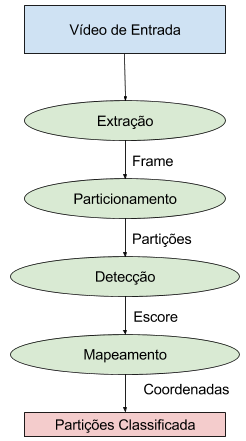
\includegraphics{etapas_metodo_proposto.png}
	\caption{Etapas do método proposto para localização de placas veiculares}
	\label{fig:etapas_metodo_proposto}
	(próprio autor).
\end{figure}

O processo “particionamento” é responsável por obter as \emph{frames} do vídeo.
Uma \emph{frame} é equivalente a uma imagem 2D, e pode ser representada por
tensores de dimensões \sigla{HWC}{Height X Width X Channel}, altura X largura X
canal} (largura, altura e canais de cor). Todos os \emph{frames} de um mesmo
vídeo geram tensores do mesmo tamanho.

O processo “fatiamento” toma como entrada uma \emph{frame} do vídeo e gera
múltiplas sub imagens aqui denominadas “partições”, geradas através de um
recorte retangular de pixels contíguos. As partições têm dimensões
compatíveis com a rede neural que será usada no passo seguinte.

A etapa denominada “detecção” é, mais especificamente, uma rede neural
artificial convolucional profunda treinada para modelar uma função escalar cujo
valor, denominado “escore”, é determinado pela presença e posição, ou não
presença, de uma placa veicular.

A etapa “binarização” estima, a partir do resultado da rede neural, se uma
partição possui uma placa de trânsito.

Este processo envolve algumas decisões que são parte fundamental da atual
proposta. Elas dizem respeito:

\begin{itemize}
\item ao tamanho das partições de imagem a serem recortadas e, por
	consequência, ao tamanho da entrada da rede neural;
\item à escolha do \emph{stride} das partições da rede neural;
\item à escolha da função que a rede neural está modelando;
\item à escolha da arquitetura e dos hiperparâmetros da rede neural.
\end{itemize}

\section{Tamanho das Partições}
O tamanho das partições define as dimensões do tensor da rede neural, portanto
o tamanho do seu “campo visual”.


\begin{figure}[!htb]
	\centering
	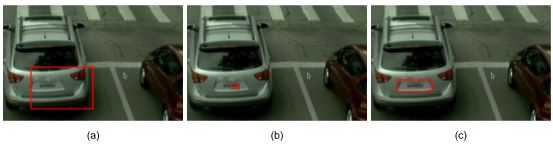
\includegraphics{ex_tres_segmentos.png}
	\caption{Exemplo de três tamanhos de partições}
	\label{fig:ex_tres_segmentos}
	Em (a) a partição possui um grande campo visual, porém tem baixa precisão.
	Em (b) há um campo visual muito pequeno para permitir que a rede neural
	opere corretamente. A terceira é apropriada, pois é relativamente pequena e
	inclui a placa inteira e vários pixels adicionais, permitindo que a rede
	neural aprenda o contraste entre placa e o fundo (próprio autor).
\end{figure}

Quanto maior o campo visual da rede neural, mais dados ela vai ter para
processar, porém menor será a precisão. Se o campo visual for muito pequeno,
como na figura \ref{fig:ex_tres_segmentos}b a precisão seria maximizada,
mas a área não é suficiente para a rede neural operar corretamente. Se
o campo visual for muito grande, como na figura \ref{fig:ex_tres_segmentos}a,
a rede neural terá mais características para usar, mas a precisão da
localização será muito prejudicada.

De forma geral, as dimensões das partições devem ser minimizadas, mas deve-se
garantir que a placa caiba no seu interior, com um pouco de
sobra. As figuras \ref{fig:ex_tres_segmentos}c e \ref{fig:ex_placa} mostram
um bom tamanho. A região adicional fora da placa vai servir para a rede
neural aprender que existe um contraste de \emph{features} entre o
interior e o exterior da placa. Este contraste vai ser usado não só para
identificar quando existe uma placa, mas também para excluir muitos casos de
falsos positivos, como \emph{banners} e outros textos que podem ser
encontrados em veículos.

\begin{figure}[!htb]
	\centering
	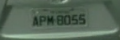
\includegraphics{ex_placa.png}
	\caption{Exemplo de partição com bom tamanho}
	\label{fig:ex_placa}
	(próprio autor).
\end{figure}

\section{\emph{Strides} das Partições}
A abordagem que está sendo proposta envolve usar um detector para construir um
localizador. Uma implementação ingênua desta abordagem seria treinar o detector
para detectar placas de trânsito que estejam centradas na sua entrada e aplicar
este detector como descrito na sessão \ref{sec:localiz_objetos}, usando
\emph{stride} $1 \times 1$.  Isso iria requerer aplicar a rede neural centrada
em cada pixel da imagem. Se for feita a aplicação de um detector com campo
visual $D_1 \times D_2$ em uma \emph{frame} com dimensões $F_1 \times F_2$
com \emph{stride} $1 \times 1$ sem estender as bordas pode-se demonstrar que
o detector terá que ser aplicado $N$ vezes, onde:

\begin{equation}
	N = (F_1 - D_1 + 1) \cdot (F_2 - D_2 + 1)
\end{equation}

Para um detector com dimensões \sigla{HW}{\emph{Height X width}, altura X
largura} de $40 \times 120$ em uma imagem
$480 \times 768$ seriam geradas 286.209 partições, e cada uma delas precisaria
ser aplicada ao detector, o que é proibitivo.

Para resolver este problema propõe-se o uso de um \emph{stride} de
$50\% \times 50\%$ do tamanho da partição. Isso significa que duas amostras
consecutivas em linha tem os seus centros a uma distância igual a sua
largura sobre dois, gerando partições como as ilustradas na figura
\ref{fig:ex_3_segmentos}.

\begin{figure}[!htb]
	\centering
	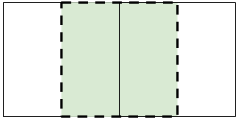
\includegraphics{ex_3_segmentos.png}
	\caption{Ilustração de 3 partições sucessivas}
	\label{fig:ex_3_segmentos}
	Observar que o centro de uma partição está contido no perímetro das
	partições vizinhas (próprio autor).
\end{figure}

Uma propriedade dessa escolha é que o centro de uma partição de imagem está
contido no perímetro de todas as partições vizinhas. Esta propriedade é
justamente o objetivo do \emph{stride} de 50\%, conforme será descrito na
sessão \ref{ses:funcao_a_modelar}.

O número de partições na direção da altura será $T_H$, e na largura será
$T_W$, sendo:

\begin{equation}
	T_H=\left\lfloor \frac{2F_1}{D_1-1} \right\rfloor \\
\end{equation}

\begin{equation}
	T_W=\left\lfloor \frac{2F_2}{D_2-1} \right\rfloor \\
\end{equation}

E o número de partições a serem classificadas será:

\begin{equation}
	N=\left\lfloor \frac{2F_1}{D_1-1} \right\rfloor \cdot
		\left\lfloor \frac{2F_2}{D_2-1} \right\rfloor
\end{equation}

Tomando o mesmo caso calculado anteriormente (detector $40 \times 120$ em
\emph{frames} $480 \times 768$ sem extensão de borda) com a estratégia proposta
de particionamento o número de partições a serem classificadas cai de 286.209
para $24 \cdot 12=288$.

\section{Função a ser Modelada} \label{ses:funcao_a_modelar}

A rede neural vai ser treinada para modelar o valor de uma função $P$ que
leva um tensor que representa uma partição da \emph{frame} a um real no
intervalo $[0;1]$:

\begin{equation}
	P:S \to [0;1] \in \mathbb{R} 
\end{equation}

O valor dessa função é resultante da presença de uma placa veicular. Devido ao
fato de que o particionamento será feito com \emph{stride} maior que 1 não há
garantia de que a placa estará centralizada, e ainda assim a função precisa
identificar que ela está presente.

A função proposta foi construída baseada na forma com que a placa veicular
passa de uma partição para a partição vizinha. A função deve possuir as
seguintes características:

\begin{itemize}
\item a função é contínua quando uma placa é movida de forma contínua na
	entrada por qualquer caminho;
\item quando a placa veicular está no centro de uma partição a função de
	saída deve ser 1, e quando está no centro da partição vizinha deve ser 0;
\item um, e apenas uma partição deve possuir valor 1 como consequência da
	presença da placa, exceto nos pontos críticos, na vizinhança dos quais a
	função é menor que 1.
\end{itemize}

A figura \ref{fig:placa_movida_entre_segmentos} ilustra os pontos principais
quando uma placa é movida horizontalmente entre duas partições.

\begin{figure}[!htb]
	\centering
	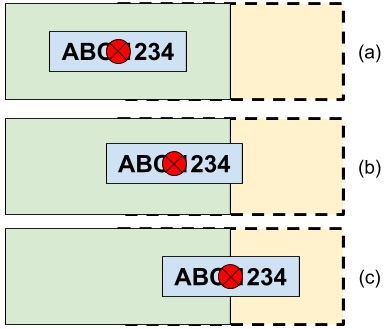
\includegraphics{placa_movida_entre_segmentos.png}
	\caption{Placa veicular sendo movida entre duas partições}
	\label{fig:placa_movida_entre_segmentos}
	Ilustração dos pontos críticos para a definição da função a ser modelada
	pela rede neural, mostrando duas partições vizinhas, uma pintada de verde e
	o outro amarelo com borda pontilhada. Em (a) a placa está centrada na
	partição da esquerda e no perímetro da partição da direita.
	Em (b) o centro da placa está no meio caminho entre os centros dos duas
	partições. Em (c) o centro da placa está no centro da partição da direita e
	perímetro da partição da esquerda (próprio autor).
\end{figure}

A figura \ref{fig:func_a_modelar_2_seg} mostra o valor da função para
duas partições vizinhas à medida que a placa é movida. Pode-se observar que
apenas um das partições possui valor 1 por vez, exceto no ponto cuja vizinhança
é menor que 1. Também observa-se
que quando a placa está centrada em uma partição, a função possui valor zero
na outra partição.

\begin{figure}[!htb]
	\centering
	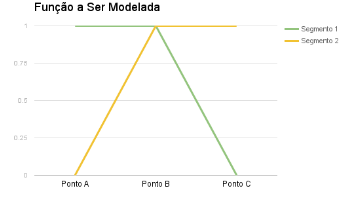
\includegraphics{func_a_modelar_2_seg.png}
	\caption{Valor da função em duas partições a medida que a placa se move
	entre elas}
	\label{fig:func_a_modelar_2_seg}
	Observa-se que valor da saída da função para duas partições a medida que a
	placa é movida do centro da partição 1 (o da esquerda) para a partição 2 (a
	da direita) (próprio autor).
\end{figure}

\begin{figure}[!htb]
	\centering
	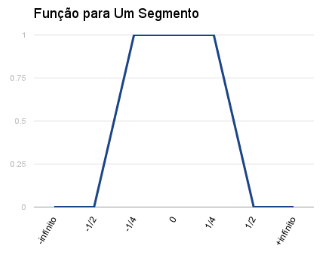
\includegraphics{func_a_modelar_1_seg.png}
	\caption{Valor da função a modelar, de $\infty$ a $+\infty$}
	\label{fig:func_a_modelar_1_seg}
	Observa-se que o valor da variável dependente a em medida que a placa
	é deslocada desde $-\infty$ até $+\infty$ da esquerda para a direita,
	enquanto a mesma está centrada na altura. A abscissa é a distância
	normalizada entre os centros da partição e da placa (próprio autor).
\end{figure}

Na figura \ref{fig:func_a_modelar_1_seg} observa-se o valor de uma função
quando a placa está alinhada na altura e é deslocada horizontalmente. Como
a abscissa é a distância normalizada entre os centros obtém-se o valor 0,5
quando o centro da placa está a uma distância igual a metade do tamanho da
partição para a direita, como ilustrado na figura
\ref{fig:placa_movida_entre_segmentos}c.

No caso de uma placa alinhada na direção $y$ (distância em $y$ é 0), e sendo
deslocada apenas em $x$, variando a distância normalizada $\Delta x$, a função
proposta é:

\begin{equation}
	f_x(\Delta x) = \begin{cases}
		1 \text{, se } |\Delta x| \leq 1/4
		\\
		\frac{1/2-|\Delta x|}{1/2-1/4} \text{, se } 1/4<|\Delta x|<1/2
		\\
		0 \text{, se } |\Delta x| \geq 1/2
	\end{cases}
\end{equation}

Da maneira semelhante, quando a distância em x é zero e a distância 
normalizada $\Delta y$ é livre:

\begin{equation}
	f_y(\Delta x) = \begin{cases}
		1 \text{, se } |\Delta y| \leq 1/4
		\\
		\frac{1/2-|\Delta y|}{1/2-1/4} \text{, se } 1/4<|\Delta y|<1/2
		\\
		0 \text{, se } |\Delta y| \geq 1/2
	\end{cases}
\end{equation}

Quando usado com as direções x e y livres a função a ser estimada pela rede
neural é:

\begin{equation} \label{eq:funcao_a_modelar}
	f=f_x \cdot f_y
\end{equation}

O gráfico \emph{3D} desta função está representado na figura
\ref{fig:func_a_modelar_3d}, mostrando o
efeito simultâneo dos eixos $x$ e $y$.  Observa-se que quando a placa
está com o seu centro a uma distância normalizada inferior 1/4 em $x$ e em $y$
simultaneamente, a função vai produzir o valor 1. O gráfico não possui
descontinuidades. Quando a distância normalizada supera 1/2 em qualquer
direção o valor da função é 0.

\begin{figure}[!htb]
	\centering
	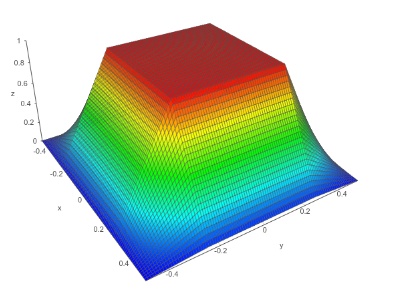
\includegraphics{func_a_modelar_3d.png}
	\caption{Gráfico 3D da função à modelar}
	\label{fig:func_a_modelar_3d}
	Gráfico da função que a rede neural deve modelar. As abscissas representam
	a distância normalizada entre o centro da partição e da placa em cada
	direção (próprio autor).
\end{figure}


\section{Arquitetura da Rede Neural}

A arquitetura da rede neural, incluindo seus hiperparâmetros, deve ser
escolhida de forma a balancear desempenho de classificação com tempo de
propagação. Se a rede neural requerer muitas operações, pode aumentar o
desempenho de classificação, mas o tempo de processamento vai aumentar.
Idealmente a rede neural deve ser restrita a um tamanho que permita que todos
as partições da imagem sejam classificadas de forma que o sistema como um todo
entregue a taxa de \emph{frames} desejada para a resolução do vídeo necessária
e hardware disponíveis onde a solução vai ser implantada.

Na implementação da rede neural convolucional existem otimizações que podem ser
feitas para reduzir o número de operações enquanto mantendo ou reduzindo pouco
a capacidade da rede neural de executar a operação para a qual vai ser
treinada. Estas otimizações são um campo ativo de pesquisa, sendo relevantes os
\emph{papers} produzidos como resultado da competição \emph{ImageNet Large
Scale Visual Recognition Competition (ILSVRC)}. Os \emph{papers}
\cite{szegedy2015going} e \cite{szegedy2015rethinking},
por exemplo, detalham várias substituições que podem ser feitas para este fim.


 % localização de placas veiculares usando cnn
%Exemplo de capitulo

\chapter{Implementação e Experimentos}

Neste capítulo será apresentada uma implementação de um sistema de localização
de imagens de veículos e os resultados das medições de desempenho do mesmo.

Também será apresentado um breve histórico mostrando algumas abordagens que
foram tentadas antes da implementação final ter sido obtida, mostrando por que
elas falharam.

\section{Arquitetura Global}
Desde as primeiras tentativas de implementação algumas características do
software permaneceram sem alterações. Isso inclui o uso de um detector para
construir um localizador e a lista de módulos de software. Estas
características são as listadas nessa seção.

Redes neurais em geral requerem grande quantidade de exemplos de treinamento
para evitar overfitting \cite{hawkins2004problem}. É crucial para o
sucesso de uma implementação acesso a dados ou a capacidade de produzi-los.

\begin{figure}[!htb]
	\centering
	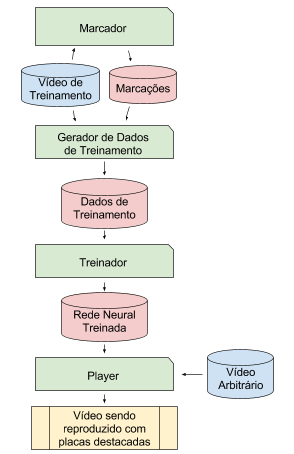
\includegraphics{cap5_arquit_global.png}
	\caption{Arquitetura Global da Implementação}
	\label{fig:cap5_arquit_global}
	Diagrama ilustrando os quatro componentes de software em verde, os vídeos
	de entrada em azul, as informações intermediárias em vermelho e a saída do
	sistema em amarelo (próprio autor).
\end{figure}

Em todas variações tentadas de implementação optou-se por gerar os dados de
treinamento. Para tal, dois softwares foram desenvolvidos: um software de
marcação manual de placas em vídeo e um software para geração desses dados.
Usando os dois softwares é possível gerar exemplos etiquetados em quantidade
suficiente no formato requerido pela rede neural. O treinamento e teste da rede
neural requereu o desenvolvimento de outros dois outros softwares. O primeiro
treina a rede neural, o segundo reproduz o vídeo enquanto aplica a rede neural
treinada, mostrando as placas identificadas. Isso resulta em quatro módulos de
software principais. O relacionamento entre eles é mostrado na figura
\ref{fig:cap5_arquit_global}.

A implementação de cada um destes módulos mudou durante a história do projeto,
porém as suas funções básicas permaneceram as mesmas.

\section{Abordagens Anteriores}
Várias tentativas de foram feitas usando abordagens incorretas durante o
desenvolvimento do projeto. O software chegou a ser implementado por completo
três vezes, sendo que só produziu resultados satisfatórios na última.

A idéia inicial para este projeto era o uso de redes neurais não-convolucionais
aplicadas diretamente aos pixels das imagens. Para tal foi escolhida a
biblioteca neuroph, devido a familiaridade e ao uso da linguagem java. A
solução foi totalmente implementada conforme arquitetura ilustrada na figura
\ref{fig:cap5_arquit_global}.

Essa implementação usava imagens em tons de cinza e segmentos com dimensões HW
$32 \times 100$ aplicadas em uma rede neural totalmente conectada com 3200
entradas e uma saída. A segmentação era feita  usando stride de 100\%, ou
seja, dois segmentos vizinhos tinham o perímetro de um dos seus lados em comum.

Esta biblioteca foi logo descartada porque o tempo de treinamento era muito
longo, impedindo a busca eficiente de configuração das camadas ocultas que
gerasse o resultado desejado. Testes com topologias mais complexas, com maior
largura e profundidade nas camadas intermediárias, chegavam a passar de uma
semana de execução. Não houve nenhuma configuração encontrada com desempenho de
classificação remotamente aceitável.

Acreditando que seria possível resolver o problema encontrando os
hiperparâmetros corretos da rede neural, e sabendo que isso requeriria
múltiplos experimentos com topologias diferentes, adotou-se a biblioteca encog,
devido ao melhor desempenho de treinamento. Essa adaptação, requereu reescrever
boa parte código. Apesar do treinamento rodar quase a uma taxa de imagens 10
vezes maior que a biblioteca anterior, também não foi encontrada topologia
com com desempenho remotamente aceitável. A figura
\ref{fig:cap5_trein_redes_nao_conv} mostra a
evolução do treinamento para algumas sessões. Entre as listadas a que teve
melhor desempenho usava 3200 neurônios na camada de entrada, então 172, 137,
109, 87, 69, 55, 44, 35 e 28 neurônios nas camadas ocultas, terminando
com uma saída.

\begin{figure}[!htb]
	\centering
	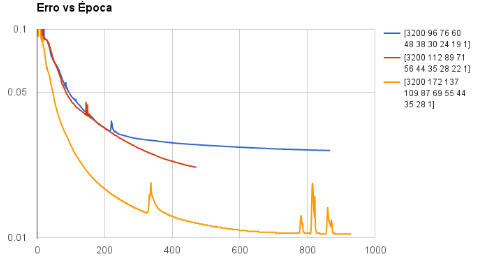
\includegraphics{cap5_trein_redes_nao_conv.png}
	\caption{Erro de treinamento de redes neurais não-convolucionais}
	\label{fig:cap5_trein_redes_nao_conv}
	A ordenada refere-se ao erro L2 calculado sem a raiz quadrada e suavizado
	usando exponential smoothing. A legenda refere-se ao número de neurônios
	em cada camada totalmente conectada (próprio autor).
\end{figure}


Quando o player era usado com as redes neurais resultantes desse treinamento o
resultado era muito ruim, com quantidade muito grande de falsos positivos.

O esquema de segmentação das imagens foi mudado de 100\% para 50\%, que é o
valor usado agora. A função que a rede neural modela foi modificada
várias vezes, mas
o resultado final, conforme visto no player, continuava ruim.

Após alguns meses a abordagem foi abandonada. Foi feita uma pesquisa sobre o
assunto descobriu-se a existência de redes neurais convolucionais. Infelizmente
a biblioteca encog e a neuroph não suportam este tipo de topologia. Também não
foram encontradas bibliotecas com grande base de usuários em java.

Neste ponto foi escolhida a biblioteca recém-lançada tensorflow. Inicialmente a
preparação dos dados de treinamento continuou sendo feita pelo código em java
que já havia sido escrito, enquanto o código de treinamento e execução foram
reescritos em python, por que era a única linguagem suportada quando essa
migração foi realizada.

O uso de duas linguagens de programação estava eliminando várias oportunidades
de reuso de código. Eventualmente o software de marcação e preparação de dados
de treinamento foi reescrito em python.

Desde os primeiros experimentos a abordagem usando redes neurais foi muito bem
sucedida.

\section{Escolha de Tecnologias}
A versão final da DCNN usa o \emph{framework} \emph{TensorFlow} do Google.
No \emph{TensorFlow} usa-se a linguagem python para descrever um ou mais
grafos onde
os nós são operações e as arestas são tensores. Uma vez que o grafo esteja
totalmente definido pode-se fornecer dados e solicitar o cálculo de qualquer
quantidade de nós. A execução em si ocorre em um runtime de alto desempenho
escrito em C++ e \emph{CUDA}, que pode ser distribuído entre múltiplas
máquinas e pode rodar em CPUs e GPUs.

A tecnologia foi escolhida por ser \emph{open source}, e por ser a ferramenta
utilizada pelo Google. Esta biblioteca é fácil de usar para pequenos projetos,
como este, e poderosa para poder escalar para sistemas com múltiplos
computadores usando GPUs de alto desempenho. Portanto adquirir conhecimento
nesta tecnologia pode ser útil para projetos futuros.

O TensorFlow permite usar python 2 ou python 3. Eu optou-se por usar a versão 3
por que é a versão mais nova da linguagem, e é a versão padrão do sistema
operacional que uso para desenvolver os projetos.

Será usado OpenCV 3 e seu wrapper python para leitura e exibição do vídeo, para
algumas operações de manipulação de imagens e para gerar a interface com
usuário. O OpenCV tem primitivos suficientes para exibir uma janela contendo
uma imagem e capturar eventos de teclado e mouse. Isso é suficiente para toda a
interface gráfica.

Tanto o wrapper python do opencv quanto o TensorFlow representam dados
numéricos, como tensores, usando uma biblioteca numérica para python chamada
numpy. Ela será usada para várias operações, como extrair sub-imagens da
\emph{frame} de vídeo que foi lida pelo opencv e fornecer estes dados para
o \emph{TensorFlow}.

Para representar as marcações que o usuário faz nos vídeos, para identificar
onde estão as placas, será usado o formato json. Este formato está se tornado o
padrão de facto para representação de dados no mercado. Além disso existem boas
bibliotecas em várias linguagens, inclusive python e java, que são minhas
linguagens principais.

O sistema operacional usado será Linux, particularmente a distribuição Arch
Linux. Eu já uso este sistema operacional no meu computador pessoal e do
escritório pelo seu sistema de atualização constante, que busca disponibilizar
o mais rápido possível as últimas versões de todos os seus componentes, como
kernel, compiladores, bibliotecas e softwares.
Arch Linux não é oficialmente suportado pelo projeto TensorFlow, mas existem
pacotes oferecidos pela comunidade tanto para versão estável quando para a
última versão git do projeto.
O servidor de código a ser usado é o git, por ser o padrão de facto do mercado.

Esse repositório já é usado pelo próprio projeto do TensorFlow.
Para edição de código será usado exclusivamente vim. Esse editor é sofisticado
e produtivo quando usado com uma linguagem como python.


\section{Recursos de Hardware}

O único recurso de hardware necessário é um computador. Como o treinamento de
redes neurais com imagens consome horas, possivelmente dias para cada sessão,
este computador idealmente seria um desktop de alto desempenho com pelo menos
uma placa de vídeo com suporte a tecnologia \emph{CUDA}.

Não foi possível ter acesso a computadores com a configuração recomendada.
Os computadores disponíveis durante a execução do projeto foram:

\begin{itemize}
\item Um notebook Core i7-3632QM com 4 cores (2 threads por core), 16 GiB
	de RAM;
\item Um notebook Core i5-4210U com 2 cores (2 threads por core), 8 GiB de RAM,
	placa de video NVidia GT-750M com 2 GiB de RAM compatível com TensorFlow.
\end{itemize}

O desenvolvimento do projeto foi quase todo feito usando o Core i7. Assim que
o suporte a GPU foi incluída no código o notebook Core i5 começou a ser usado,
e, a partir deste ponto, ambos os coputadores passarm a ser usados.

\section{Implementação dos Módulos de Software}

Nesta seção está detalhada a implementação de cada módulo de software.

\subsection{Marcador}

\begin{figure}[!htb]
	\centering
	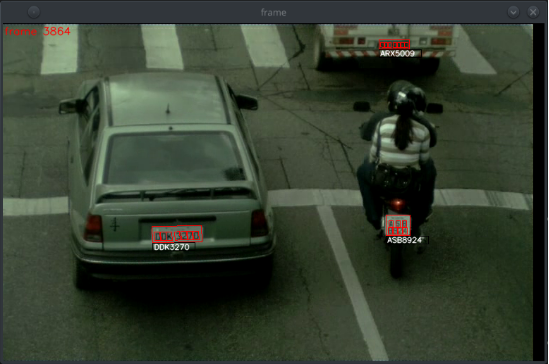
\includegraphics{cap5_tela_marcador.png}
	\caption{Interface com usuário do \emph{Marcador}}
	\label{fig:cap5_tela_marcador}
	A tela está mostrando 3 veículos marcados (próprio autor).
\end{figure}

O software marcador foi construído como um script python que recebe o nome de
um arquivo de vídeo como parâmetro. Ele permite:

\begin{enumerate}
\item Reproduzir o vídeo;
\item Pausar a reprodução do vídeo
\item Avançar / voltar frame-a-frame;
\item Saltar para uma \emph{frame} digitando-se o número dela;
\item Quando o vídeo está em pausa, permite clicar no vídeo para adicionar um
	marcador de placa;
\item Usar o teclado para mover, rotacionar e alterar o marcador, de forma que ele
	circule corretamente a placa sendo marcada;
\item Digitar o número da placa veicular
\end{enumerate}

Como pode ser visto na figura \ref{fig:cap5_tela_marcador}, o software
marcador permite marcar placas de
carros e motos, e é possível identificar o número da placa. Isto tem como
objetivo permitir que as mesmas marcações possam ser usadas futuramente para
fazer OCR das placas. As marcações são salvas em um arquivo \emph{json}.

Quando uma \emph{frame} possui pelo menos uma placa veicular marcada todo
o resto da
imagem vai ser considerado pelo software de treinamento como região sem placa.
Por isso, se uma placa for marcada em uma \emph{frame}, deve-se marcar todas as
placas.

\begin{table}
	\center
	\caption{Arquivos de vídeo usados durante o desenvolvimento}
	\renewcommand{\arraystretch}{1.6}
	\begin{tabular}{ccccc}
		\Xhline{6\arrayrulewidth}
		\textbf{Vídeo} &
			\textbf{Resolução} &
			\textbf{FPS} &
			\textbf{Tamanho} &
			\textbf{Duração} \\
		\Xhline{2\arrayrulewidth}
		video1.avi & $480 \times 768$   & 25,0 & 141 MiB & 8:27  \\
		video2.avi & $1080 \times 1920$ & 25,0 & 1,0 GiB & 36:16 \\
		video3.avi & $1080 \times 1920$ & 25,0 & 465 MiB & 8:02  \\
		\Xhline{6\arrayrulewidth}
	\end{tabular}
	\label{tbl:videos}
\end{table}

Todo o desenvolvimento foi feito usando três vídeos. As características dos
vídeos estão listadas na tabela \ref{tbl:videos}, e uma \emph{frame} de
cada vídeo está mostrada na figura \ref{fig:cap5_3_videos}.

\begin{figure}[!htb]
	\centering
	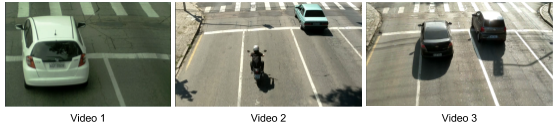
\includegraphics{cap5_3_videos.png}
	\caption{Uma \emph{frame} de cada vídeo usado durante o desenvolvimento}
	\label{fig:cap5_3_videos}
	(próprio autor).
\end{figure}

A tabela \ref{tbl:marc_videos} mostra a quantidade de marcações feitas em cada
vídeo. A maior parte das marcações foram feitas no \emph{video1}.

\begin{table}
	\center
	\caption{Marcações feitas em cada vídeo}
	\renewcommand{\arraystretch}{1.6}
	\begin{tabular}{c c c}
		\Xhline{6\arrayrulewidth}
		\textbf{Vídeo} &
			\textbf{Quadros Marcados} &
			\textbf{Placas Marcadas} \\
		\Xhline{2\arrayrulewidth}
		video1.avi & 191 & 233 \\
		video2.avi & 71  & 71  \\
		video3.avi & 0   & 0   \\
		\Xhline{6\arrayrulewidth}
		TOTAL      & 262 & 304 \\
	\end{tabular}
	\label{tbl:marc_videos}
\end{table}

\subsection{Gerador de Dados de Treinamento}

\begin{figure}[!htb]
	\centering
	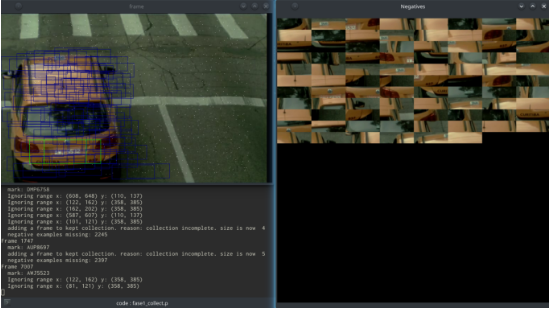
\includegraphics{cap5_tela_gerador.png}
	\caption{Interface gráfica do gerador de dados}
	\label{fig:cap5_tela_gerador}
	A imagem da esquerda mostra o quadro que está sendo processado e mostra as
	regiões onde os exemplos negativos estão sendo coletados. A imagem da
	direita mostra os próprios exemplos negativos que estão sendo enviados para
	o arquivo (próprio autor).
\end{figure}

O software gerador de dados de treinamento também recebe como parâmetro o nome
do arquivo de vídeo onde vai operar, e vai abrir este arquivo de vídeo e as
marcações feitas nele. Este software roda de modo não-interativo,
terminando sem intervenção do usuário quando a geração do set de
treinamento está concluída. A interface gráfica está ilustrada na figura
\ref{fig:cap5_tela_gerador}

O set de treinamento é armazenado em formato binário contendo registros de
tamanho fixo. Cada registro contém a imagem seguida de um \emph{label}. A
imagem é codificada no formato HWC usando 1 byte por canal de cor,
sendo a cor na ordem RGB. O \emph{label} representa o valor que a rede neural
deve aprender (float de 0 à 1), mas é codificado como um inteiro de
8 bits sem sinal.  Como a imagem é $40 \times 120 \times 3$ e o \emph{label}
tem 1 byte, então cada registro possui 14401 bytes.

Este software vai iniciar tomando a lista de \emph{frames} marcadas em
uma ordem
aleatória. Então vai coletar exemplos de placas veiculares centradas e fora
de centro e exemplos de imagens que não contém placas, e vai salvá-las no
arquivo de saída. A cada um dos exemplos de treinamento este software
também salva um número que é o valor da função que a rede neural deve
produzir para esta placa, conforme equação \ref{eq:funcao_a_modelar}.

Tomando uma placa nas coordenadas $y \times x$, o software primeiro gera um
recorte centrado nessas coordenadas e com o tamanho $40 \times 120$. Este
tamanho é definido em um arquivo de configuração. Todos os exemplos
coletados desta forma recebem o \emph{label} 1 (codificado como 255).

Para coletar os exemplos de placas não centralizadas coleta-se recortes de
aproximadamente 4 em 4 \emph{pixels} dentro de uma região próxima da placa. O
algoritmo avança precisamente na taxa de 4 \emph{pixels}, porém adiciona um
número aleatório de -2 à 2 em cada um deles. Isso tem como objetivo evitar de
fornecer dados muito regulares para a rede neural para evitar que ela
aprenda algum truque relacionado à este padrão de distância. A região onde
coleta-se estes exemplos é tal que o centro fica dentro de uma região
$40 \times 120$ centrada na placa do veículo, como ilustrado na figura
\ref{fig:cap5_regiao_coleta_amostras}.

\begin{figure}[!htb]
	\centering
	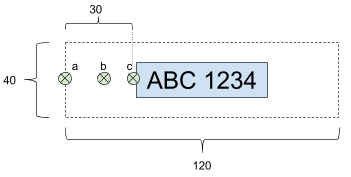
\includegraphics{cap5_regiao_coleta_amostras.png}
	\caption{Região onde amostras são coletadas}
	\label{fig:cap5_regiao_coleta_amostras}
	Esta região delimita os centros dos Segmentos, então pixels fora dessa
	região são coletados.  Segmentos centrados dentro da região delimitada são
	coletados de 4 em 4 pixels, sendo que cada uma dessas regiões é deslocada 2
	pixels para a direita ou para a esquerda. Em verde estão marcados três
	pontos, a, b e c, que serão atribuídos respectivamente aos \emph{labels} 0,
	$^1/_2$ e 1 (próprio autor).
\end{figure}

A região delimitada é exatamente a região na qual o valor é não-zero. O ponto
(c) na figura \ref{fig:cap5_regiao_coleta_amostras} mostra o limiar que está
a $^1/_4$ de distância do centro na direção da largura. Neste ponto a função
começa a decair de 1 para 0 (que são codificados como 255 e 0). O ponto (a)
é onde a função atinge o valor 0, e o ponto (b) está precisamente no
meio do caminho, possuindo o valor 0,5 (codificado como 128).

Após coletar os exemplos de placas contidas na região acima indicada ocorre a
coleta de imagens  fora da região, denominada coleta de “exemplos negativos”. A
todos os exemplos coletados dessa maneira é atribuído o \emph{label} 0.

O algorítmo que coleta esses exemplos passou por vários aprimoramentos. A
versão final, que vai ser descrita, melhorou consideravelmente o desempenho do
treinamento comparado com as versões iniciais.

A primeira, e mais importante otimização foi a eliminação de exemplos
parecidos. Quando se coleta exemplos de regiões da imagem que não são placas de
carro pode-se acabar obtendo um recorte que inclui apenas o asfalto. Se outro
recorte for feito em outra \emph{frame} na mesma região pode acabar sendo
um exemplo muito parecido, como ilustrado na figura
\ref{fig:cap5_coleta_negativa_igual}.

\begin{figure}[!htb]
	\centering
	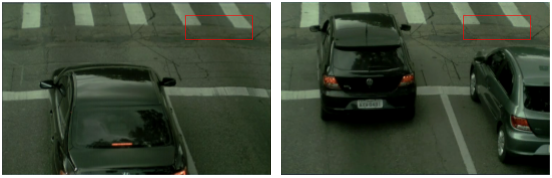
\includegraphics{cap5_coleta_negativa_igual.png}
	\caption{Exemplo de duas regiões iguais em frames diferentes}
	\label{fig:cap5_coleta_negativa_igual}
	As regiões possuem as mesmas coordenadas, e contém pixels de fundo da
	imagem (próprio autor).
\end{figure}

Por este motivo o software mantém as últimas 100 \emph{frames} processadas.
Quando um “exemplo negativo” vai ser coletado em uma região a imagem é
comparada com os
pixels da mesma região nestas frames que foram armazenadas. O critério de
comparação é:

\begin{equation}
	d_C=\frac{1}{N} \sum_{n=1}^N \sqrt{\left| R_C [n] -I_C [n] \right|}
\end{equation}

Onde $R_C[n]$ é o valor do canal de cor “C” do n-ésimo píxel do segmento de
referência, e $I_C[n]$ é o mesmo canal do n-ésimo pixel do
segmento que está sendo testado. Quando o valor da média dessa métrica
para os três canais é menor que $\sqrt{8}$ as imagens são consideradas
semelhantes, e a amostra é recusada. Foram
testadas métricas, como média do módulo da diferença, e média da diferença
quadrática, mas tiveram desempenho inferior ao serem comparados usando a
percepção humana como referência. A figura
\ref{fig:cap5_tela_gerador} mostra o efeito desta otimização.
Cada retângulo azul mostra a região onde um exemplo negativo foi coletado.
Observa-se que o asfalto não está sendo coletado.

A segunda otimização foi a distância entre duas amostras negativas. Duas
amostras muito próximas tem pouco valor para treinamento da rede neural devido
à invariância a deslocamento. Por isso, para uma amostra ser aceita como
“exemplo negativo” ela precisa estar a mais de 4 pixels de todos os outros
exemplos coletados.

A terceira otimização foi o processo de escolha das coordenadas onde os
exemplos são coletados. Inicialmente usava-se um grid regular, mas essa
abordagem acabava coletando uma quantidade muito grande de exemplos negativos.

Como isso a rede neural acabava aprendendo a favorecer valores negativos, pois
errar “para mais” acabava sendo punido mais severamente que errar “para menos”
durante a otimização. Para poder balancear a quantidade de exemplos negativos e
positivos foi necessário substituir o grid linear, já que ele favorecia coletar
exemplos negativos na parte superior da imagem, pois a coleta terminava antes
da imagem chegar na parte inferior.

Para resolver isso foi adotado um processo que escolhe coordenadas usando uma
distribuição uniforme e testa se nas coordenadas existe um exemplo negativo
válido. Infelizmente este algoritmo é $O(\infty)$ no pior caso. Por isso um
novo algoritmo de busca
que tem probabilidade próxima de uniforme para a busca, vai sempre encontrar
todas as soluções, e sempre termina precisou ser criado. Este algoritmo é uma
modificação do BFS (\emph{breadth-first search}), no no qual a ordem na
qual a busca é adicionada à pilha é aleatória. O algoritmo pega
de uma pilha uma região
retangular na qual deve encontrar pontos válidos e usa um gerador aleatório
uniforme para escolher coordenadas e testar. Se o teste falhar divide a região
em duas sub-regiões na direção onde a imagem for maior (altura ou largura) e
adiciona as regiões na pilha em ordem aleatória. Cada vez que coordenadas
válidas são encontradas elas são adicionadas na lista de resposta. Se a lista
possui o número solicitado de respostas o algoritmo termina, caso contrário
continua.

\begin{table}
	\center
	\caption{Exemplos de treinamento gerados para cada vídeo}
	\renewcommand{\arraystretch}{1.6}
	\begin{tabular}{c c c p{2.5cm} p{2.5cm}}
		\Xhline{6\arrayrulewidth}
		\textbf{Entrada} &
			\textbf{Saída} &
			\textbf{Tamanho} &
			\textbf{Registros \newline Gerados} \\
		\Xhline{2\arrayrulewidth}
		video1.avi & video1.nn1.bin & 1,1 GiB  & 64.714  \\
		video2.avi & video2.nn1.bin & 901 MiB  & 89.672  \\
		\Xhline{6\arrayrulewidth}
		TOTAL      &                & 2,07 GiB & 154.386 \\
	\end{tabular}
	\label{tbl:marc_videos}
\end{table}

Um script escrito em bash foi escrito partir um arquivo destes em arquivos
menores, contendo 128 amostras cada. Isso gerou 630 arquivos a partir de
\emph{video1.nn1.bin} e 240 arquivos a partir de \emph{video2.nn1.bin}.

Finalmente, um diretório foi criado contendo links simbólicos para todos os 869
arquivos. Este diretório é o resultado final da geração de exemplos, e contém
todas as amostras coletadas de todos os vídeos.

\subsection{Treinador}

\begin{figure}[!htb]
	\centering
	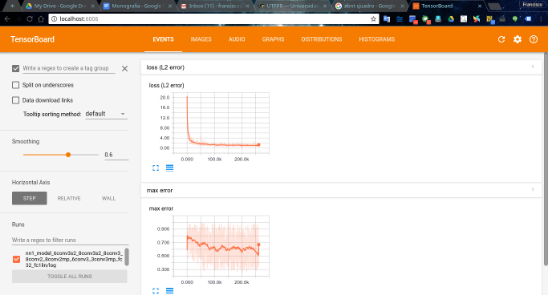
\includegraphics{cap5_tela_treinador.png}
	\caption{Página do \emph{TensorBoard} mostrando progresso do treinamento}
	\label{fig:cap5_tela_treinador}
	Esta é uma página \emph{web} que permite observar a evolução do
	treinamento (próprio autor).
\end{figure}

O treinador é um módulo de software onde se configura uma topologia de rede
neural convolucional, que é treinada usando os dados produzidos pelo gerador de
dados de treinamento.

Para realizar o treinamento tanto da rede neural um grafo apresentado na figura
\ref{fig:cap5_grafo_treinamento} foi construído.

\begin{figure}[!htb]
	\centering
	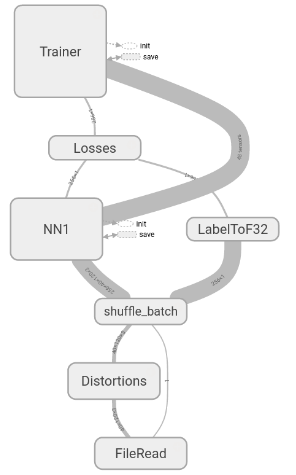
\includegraphics{cap5_grafo_treinamento.png}
	\caption{Grafo usado para treinamento da rede neural convolucional}
	\label{fig:cap5_grafo_treinamento}
	Esta imagem mostra o grafo do \emph{TensorFlow} usado para treinar
	a rede neural, que é o bloco \emph{NN1} (próprio autor).
\end{figure}

O bloco “FileRead” possui uma lista com todos os arquivos de treinamento
gerados pelo gerador de exemplos de treinamento. Essa lista é embaralhada, e
então cada um dos registros é lido em sequência. A imagem é representada por um
tensor de inteiros de 8 bits com dimensões $40 \times 120 \times 3$, e o
label da imagem é representado com um tensor unidimensional com dimensão $1$.

Como a rede neural está sendo treinada usando apenas dois vídeos existe o risco
da rede neural treinada fique muito sensível a fatores como a iluminação. Para
impedir que isso aconteça as imagens são distorcidas durante o treinamento no
bloco de distorções, que está ilustrado na figura \ref{fig:cap5_distorcao}.
A imagem é convertida para ponto-flutuante com canais no intervalo $[0;1]$,
conforme requerido pelos primitivos do próprio \emph{TensorFlow}.
No final das distorções a imagem é convertida
novamente para inteiro de 8 bits por canal. O motivo para isso é fazer com o
que o bloco “NN1”, que implementa a rede neural seja o mais otimizado possível
para classificar imagens, não tanto para treinamento.

\begin{figure}[!htb]
	\centering
	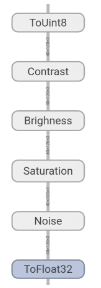
\includegraphics{cap5_distorcao.png}
	\caption{\emph{Pipeline} de distorção de imagens}
	\label{fig:cap5_distorcao}
	A imagem é convertida para ponto-flutuante com cada canal no intervalo
	$[0;1]$, é adicionado ruído normal, a saturação, brilho e contraste são
	alterados conforme uma distribuição normal. O número é então convertido
	novamente para inteiro de 8 bits por canal (próprio autor).
\end{figure}

O bloco “Noise” adiciona ruído normal à imagem somando-a com um tensor com as
mesmas dimensões onde o valor de cada canal é gerado por uma distribuição
normal de média 0 e desvio padrão 0,06.

O bloco “Saturation” altera a saturação entre 0,2 a 1,5, sendo que 1 representa
manter a saturação inalterada. O bloco “Brightness” faz uma alteração no brilho
aumentando ou diminuindo em até 40\%. O bloco “Contrast” faz uma alteração de
contraste entre 0,6 e 1,4, sendo que 1 representa manter o brilho. As escolha
do valor em todos os casos é aleatória de acordo com distribuição uniforme.

O resultado das distorções, juntamente com o label da imagem são fornecidos
para o bloco “shuffle\_batch”. Este bloco tem a função de embaralhar os
dados e agrupar imagens em batches. Este bloco usa 8 threads para consumir
os dados dos blocos anteriores, o que significa que leitura e shuffling vai
ocorrer em paralelo. Quando 2560 imagens são lidas elas são embaralhadas
elas são agrupadas em batches de 256 imagens, gerando tensores com
dimensões $256 \times 40 \times 120 \times 3$. Como cada arquivo contém
128 imagens, então as imagens
sendo lidas contém, no pior caso um set aleatório de imagens de 20
arquivos. Os arquivos em sí são lidos em ordem aleatória, o que gera uma
amostragem razoavelmente diversa das informações de entrada.

Quanto maior o tamanho do batch maior a precisão da estimativa de erro,
portanto este número é o maior possível suportado pelo hardware onde o
treinamento está sendo realizado.

Se o treinamento for rodado por tempo suficiente, todas as imagens serão
lidas. Se o treinador precisar de mais exemplos as mesmas imagens serão lidas
novamente, em ordem diferente. Porém, graças ao sistema de distorção de
imagens que é parte do pipeline de leitura, uma mesma imagem lida múltiplas
vezes muito provavelmente não chegará idêntica na rede neural.

Os tensores que saem do shuffler são fornecidos a rede neural, que está no
bloco “NN1”, que está ilustrado na figura \ref{fig:cap5_cnn}.

\begin{figure}[!htb]
	\centering
	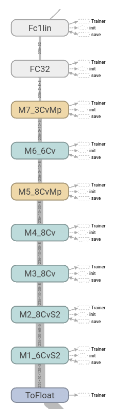
\includegraphics{cap5_cnn.png}
	\caption{Pipeline descrevendo a rede neural convolucionao profunda}
	\label{fig:cap5_cnn}
	(próprio autor)
\end{figure}

Pode-se ver pela espessura das linhas que conectam os blocos que a quantidade
de informação reduz ligeiramente em cada etapa. Como a rede neural precisa
de um tempo de propagação baixo algumas técnicas foram usadas para
reduzir o número de computações.

A primeira estratégia é a redução agressiva do tamanho dos tensores nas duas
primeiras camadas, inspirado em \cite{szegedy2015going}. \emph{Stride} é usado
para fazer um resampling da imagem. Este método usa mais CPU do que resampling
por métodos como bilinear, porém permite acesso à textura da imagem original. A
primeira camada usa um kernel de $2 \times 2$ ao invéz de $3 \times 3$,
reduzindo o número de multiplicações de 9 para 4.

Não está sendo usada nenhuma convolução maior que $3 \times 3$.
\cite{szegedy2015going} defende que, pelo menos em alguns casos,
convoluções $5 \times 5$ podem ser substituídas por duas convolução
sucessivas $3 \times 3$ enquanto reduz o número de
multiplicações de $25$ para $2 \cdot 9=18$.

\begin{table}
	\center
	\caption{Camadas da Rede Neural Implementada}
	\renewcommand{\arraystretch}{1.6}
	\begin{tabular}{c c c c}
		\Xhline{6\arrayrulewidth}
		\textbf{Nome} &
			\textbf{Tensor de Entrada} &
			\textbf{Operação} &
			\textbf{DOF} \\
		\Xhline{2\arrayrulewidth}
		M1 & $256 \times 40 \times 120 \times 3$ & 6 cv2x2 s2x2 relu  & 78   \\
		M2 & $256 \times 20 \times 60 \times 6$  & 8 cv3x3 s2x2 relu  & 440  \\
		M3 & $256 \times 10 \times 30 \times 8$  & 8 cv3x3 relu       & 584  \\
		M4 & $256 \times 10 \times 30 \times 8$  & 8 cv3x3 relu       & 584  \\
		M5 & $256 \times 10 \times 30 \times 8$  & 8 cv3x3 relu mp2x2 & 584  \\
		M6 & $256 \times 5  \times 15 \times 8$  & 6 cv3x3 relu       & 438  \\
		M7 & $256 \times 5  \times 15 \times 6$  & 3 cv3x3 relu mp2x2 & 165  \\
		-  & $256 \times 3  \times 8 \times 3$   & flatten            & 0    \\
		FC32 & $256 \times 72$                   & fc32 relu          & 2.336\\
		FC1 & $256 \times 32$                    & fc1 linear         & 33   \\
		SAÍDA & $256$                            &                    &      \\
		\Xhline{6\arrayrulewidth}
		TOTAL & & & 5.242 \\
	\end{tabular}
	\label{tbl:marc_videos}
\end{table}

Nas últimas camadas está sendo usado maxpool $2 \times 2$. Esta estratégia é
computacionalmente mais cara que usar convolução com stride maior que 1, pois
de cada 4 valores 3 deles são descartados. Como as imagens são menores no final
da rede neural optou-se pela operação mais cara. O efeito em tempo de
propagação é negligenciável, o efeito na qualidade da detecção não foi medido.

Outro ponto importante é o controle do número de graus de liberdade. Os
primeiros modelos tinham mais de 50.000 graus de liberdade, e este valor foi
reduzido para 5.242. Menos parâmetros implica várias vantagens, como
treinamento mais rápido, menos uso de memória, capacidade de usar
\emph{batches} maiores e menor chance de \emph{overfitting}.

O processo que mais ajudou a aprimorar sucessivamente os hiperparâmetros da
rede neural foi procurar uma rede neural com menos parâmetros que tenha
desempenho comparável. Quando esta estratégia foi adotada a produtividade no
que diz respeito a otimização destes parâmetros teve um salto considerável.

A saída da rede neural, denominado “A”, é um tensor contendo um valor para cada
uma das imagens, portanto um com dimensão 256. Para o treinamento a saída da
rede neural vai ser comparado com os labels que estavam nos dados de
treinamento, representado pelo tensor “B”, e também forma um tensor
monodimensional com dimensão 256. O erro entre as duas medidas é mapeado para
um único escalar, denominado perda, ou loss, pela metade da normal L2 entre os
dois tensores sem a raíz quadrada:

\begin{equation}
	loss=\frac{1}{2} \sum_{n=1}^N \left( A[n] - B[n] \right)^2
\end{equation}

Esta medida foi usado porque é calculada eficiente pelo \emph{TensorFlow}
através da função \textbf{tf.nn.l2\_loss(t, name=None)}. O software de
treinamento usa um otimizador
Adam \cite{kingma2014adam} para atualizar os parâmetros treináveis da rede
neural de forma a minimizar este valor.

As figuras \ref{fig:cap5_train_histogram} e \ref{fig:cap5_erro_treinamento}
mostram a evolução do treinamento durante uma sessão de 25
horas treinadas em um notebook Core i5 usando GPU. Durante este tempo foram
consumidos mais de 66 milhões de imagens, o que consumiu todos os 2 GiB de
dados e seus 154.386 exemplos de imagens cerca de 428 vezes.

\begin{figure}[!htb]
	\centering
	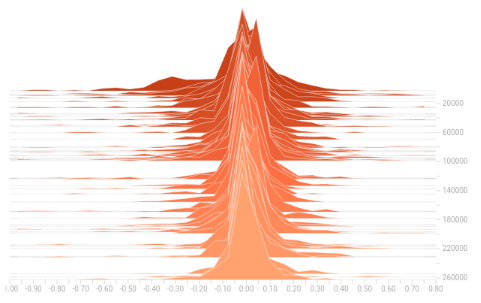
\includegraphics{cap5_train_histogram.png}
	\caption{Histograma temporal do erro classificação}
	\label{fig:cap5_train_histogram}
	Pode-se observar os erros se concentrando cada vez mais próximo de 0 a
	medida que o treinamento avança. A escala indicada são batches de 256
	imagens, portanto este gráfico o resultado após mais de 66 milhões de
	imagens (próprio autor).
\end{figure}

\begin{figure}[!htb]
	\centering
	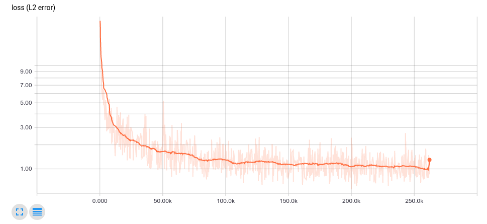
\includegraphics{cap5_erro_treinamento.png}
	\caption{Gráfico do erro de treinamento}
	\label{fig:cap5_erro_treinamento}
	Evolução da função de perda que o otimizador está minimizando, amortecido
	usando método média local. A abscissa é o número do batch, e cada batch
	possui 256 imagens (próprio autor).
\end{figure}

\subsection{Player}

\begin{figure}[!htb]
	\centering
	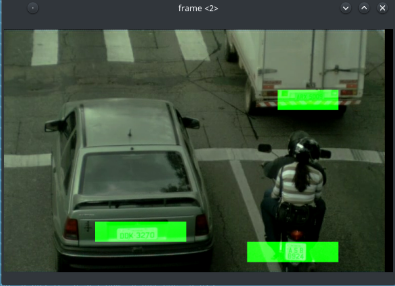
\includegraphics{cap5_tela_player.png}
	\caption{Interface com o usuário do módulo \emph{Player}}
	\label{fig:cap5_tela_player}
	No momento que a tela foi capturada o software está exibindo um vídeo
	enquanto destaca as placas que está localizando (próprio autor).
\end{figure}

O quarto módulo de software usa a rede neural treinada para reproduzir o
conteúdo de um vídeo ou da câmera enquanto destaca as placas de carros
localizadas. A figura \ref{fig:cap5_tela_player} mostra a interface do usuário
no momento em que está exibindo um vídeo quando três veículos estão passando.
As placas dos mesmos estão sendo destacadas.

O software implementa o método de classificação proposto nesta monografia por
completo. O método de binarização é um limiar simples em 0,75. Este valor
permite que quando a placa está transitando de um segmento para outro ambas as
placas serão iluminadas momentaneamente antes da placa que ficou para trás
apagar.

Não foi implementado nenhum método para usar a correlação temporal das
informações coletadas.

Para o \emph{video1.avi} a rede neural é executada 288 vezes para frame do
vídeo, sendo que uma linha completa contendo 12 segmentos é fornecido para a
rede neural por vez.

O software é capaz de operar em qualquer vídeo que possa ser lido pelo
\emph{opencv3} e pode usar a imagem da câmera do computador.

\section{Experimentos e Desempenho}

Para os testes de tempo de classificação foi usado o módulo “player”. Este
módulo mostra uma janela com o vídeo sendo classificado enquanto envia para
stdout uma série de informações de desempenho. Estes dados foram usados nas
medições relacionadas a tempo de classificação.


\begin{table}
	\center
	\caption{Taxa de Frames por Segundo}
	\renewcommand{\arraystretch}{1.6}
	\begin{tabular}{ccccc}
		\Xhline{6\arrayrulewidth}
		\textbf{Vídeo} &
			\textbf{Resolução} &
			\textbf{FPS (GPU)} &
			\textbf{FPS (CPU)} &
			\textbf{Melhoria} \\
		\Xhline{2\arrayrulewidth}
		camera     & $480  \times 640$  & 15,8 & 9.12 & 73\%  \\
		video1.avi & $480  \times 768$  & 14,8 & 8,08 & 84\%  \\
		video2.avi & $1080 \times 1920$ & 3,29 & 1,51 & 117\% \\
		video3.avi & $1080 \times 1920$ & 3,34 & 1,51 & 121\%  \\
		\Xhline{6\arrayrulewidth}
	\end{tabular}
	\label{tbl:player_fps}
\end{table}

Observa-se na tabela \ref{tbl:player_fps} que o “player” não consegue
atingir a taxa de 25 frames por segundo
de nenhum dos três vídeos, mesmo com uso de GPU. A taxa de frames
aumenta consideravelmente quando a GPU é usada. Entre os casos
testados o ganho é maior quando a resolução do vídeo aumenta. A figura
\ref{fig:cap5_player_fps} mostra o resultado em forma de gráfico.

\begin{figure}[!htb]
	\centering
	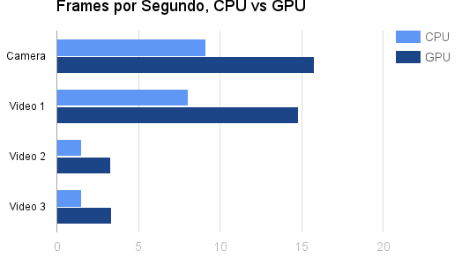
\includegraphics{cap5_player_fps.png}
	\caption{Taxa de frames por segundo no módulo \emph{Player}}
	\label{fig:cap5_player_fps}
	Gráfico mostrando desempenho em frames por segundo para localizar placas na
	câmera VGA do computador, e nos três vídeos. Maior é melhor (próprio
	autor).
\end{figure}

O player envia para o stdout o tempo gasto em cada uma das tarefas durante o
processamento da frame. Coletando-se estes dados e calculando-se as médias do
tempo gasto em cada tarefa foi gerado o gráfico na figura X.

\begin{figure}[!htb]
	\centering
	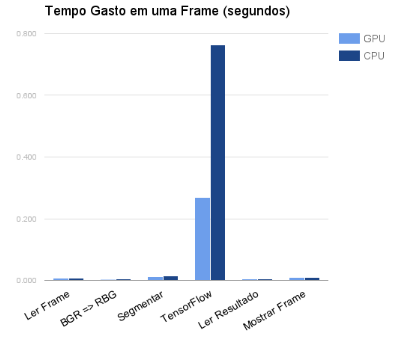
\includegraphics{cap5_frame_benchmark.png}
	\caption{Tempo gasto em cada subtarefa no processamento de uma
		\emph{frame}}
	\label{fig:cap5_frame_benchmark}
	Gráfico mostra que, ao processar um vídeo $1080 \times 1920$ a grande
	maioria do tempo é gasto executando o grafo do \emph{TensorFlow}. Outras
	tarefas executadas pelo código em \emph{Python} consomem um percentual
	pequeno do tempo da frame (próprio autor).
\end{figure}

Pode-se ver claramente que a vasta maioria do tempo é gasta executando os
grafos do \emph{TensorFlow}. Também foi possível confirmar que o ganho do
desempenho no caso do uso do GPU foi consequência do \emph{TensorFlow}
consumir menos tempo para executar. Observou-se que na implementação CPU
o \emph{TensorFlow} tomou 94,9\% do tempo de processamento da frame, e no
caso que usa GPU tomou 88,1\%.
 % implementacao e experimentos
%Exemplo de capitulo

\chapter{Conclusões}

Os resultados obtidos mostram que o método proposto é capaz de localizar placas
veiculares com excelentes valores de \emph{precision} e \emph{recall}.  
A rede neural reproduz corretamente o valor da função
que está modelando, estimando a posição da placa veicular na sua
entrada, apesar de ter sido treinada com substancial adição de ruído e outras
distorções, demonstrando a validade do método.

O método de particionamento usado para determinar onde a rede neural é
aplicada, não foi suficiente para permitir atingir taxa de \emph{frames}
nominal de nenhum dos vídeos usados no computador testado. O aumento da
taxa de \emph{frames}
pode ser conseguido de várias formas, incluindo o uso de uma GPU mais rápida,
otimização da topologia da rede neural, melhor agendamento de lotes e melhor
distribuição de tarefas para CPU e GPU.

Uma consequência negativa do método de particionamento usado
é a imprecisão na
posição da placa. O algorítimo usado para converter os escores para coordenadas
usou ``máxima local'', e por isso, quando uma placa é localizada, a posição real
dela pode estar $\pm 20 \times \pm 60$ \emph{pixel}, o que pode ser excessivo
para
certas aplicações. No entanto é possível reduzir pela metade com um método mais
sofisticado de conversão dos escores em coordenadas usando os quatro maiores
valores. Se houver \emph{budget} computacional é possível também
aproximar mais as partições, reduzindo arbitrariamente estes valores.

Para futuros trabalhos sugere-se adicionar ao modelo aqui proposto a
capacidade de fazer segmentação e OCR, de forma a produzir um sistema completo
de identificação de placas veiculares. Dois aspectos do método proposto que
podem ser melhorados são a função modelada pela rede neural, que é $C0$ e
poderia ser $C1$ para melhorar a regressão, e o processo de cálculo de
coordenadas das placas a partir dos escores da rede neural que poderia
aumentar a precisão da localização.  Entre os aspectos práticos, e de
implementação, sugere-se continuar o trabalho de otimização da rede
neural para reduzir a quantidade de computações sem gerar muito impacto nos
resultados de classificação.

 % conclusões

%--------------------------------------
%Elementos Pós-Textuais
%--------------------------------------

%Bibliografia, gerada automaticamente a partir do arquivo .bib em conjunto com as citações presentes no texto.
\bibliography{bib/bibliografia}

%Apendices. Use caso necessário. Todos capítulos após o comando \apendice serão tratados como Apêndices. 
%\apendice
%\chapter{Titulo do Ap\^endice}

\begin{table}
	\center
	\caption{Tabela com \emph{Bias} aprendidos durante o treinamento}
	\renewcommand{\arraystretch}{1.6}
	\begin{tabular}{c p{8.0cm}}
		%\toprule
		\Xhline{6\arrayrulewidth}
		\textbf{Camada} &
			\textbf{Bias} \\
		\Xhline{2\arrayrulewidth}
		%\midrule
		M1 & [
			0.09098341  0.06582655 0.07168961  0.04435913  0.88525242
			 0.040886  ] \\
		M2 & [
			0.06287824  0.27774701 0.4061453  -1.30334198 0.06711841
			-0.11221329 0.06533439  1.06334031] \\
		M3 & [
			-0.22721343 -0.17090347 0.11291317 0.15302791 0.08438433
			0.02150897 0.20345436 -0.15001012] \\ 
		M4 & [
			0.71632427 0.06480201 -0.04017521 0.58979249 0.08649875
			0.25791088 -0.08067521 -0.21774861] \\
		M5 & [
			-0.47191876 -0.34982765 0.20474097 0.30674952 -0.0380516
			0.08939933 0.08481776 0.40020576] \\
		M6 & [
			0.57687277 1.21591604 0.21532156 -0.1975698 0.97217804
			1.23713207] \\
		M7 & [
			0.23965664 0.70356482 0.20452037] \\
		
		\Xhline{6\arrayrulewidth}
	\end{tabular}
	\label{tbl:player_fps}
\end{table}


%\chapter{Titulo do Outro Ap\^endice}

Isto \'e um exemplo de Ap\^endice (b).



%Anexos. Use caso necessário. Todos capítulos após o comando \anexo serao tratados como Anexos. 
%\anexo
%\chapter{Titulo do Anexo}

Isto \'e um exemplo de Anexo.


%\chapter{Titulo do Outro Anexo}

Isto \'e um exemplo de Anexo (b).



\end{document}
